\documentclass[sigconf, authorversion, nonacm, screen]{acmart}
%%
%% \BibTeX command to typeset BibTeX logo in the docs
\AtBeginDocument{%
  \providecommand\BibTeX{{%
Bib\TeX}}}

%% Rights management information.  This information is sent to you
%% when you complete the rights form.  These commands have SAMPLE
%% values in them; it is your responsibility as an author to replace
%% the commands and values with those provided to you when you
%% complete the rights form.

%\setcopyright{acmlicensed}
%\copyrightyear{2025}
%\acmYear{2018}
%\acmDOI{XXXXXXX.XXXXXXX}

%% These commands are for a PROCEEDINGS abstract or paper.

%\acmConference[Conference acronym 'XX]{Make sure to enter the correct
%  conference title from your rights confirmation email}{June 03--05,
%  2018}{Woodstock, NY}

%%
%%  Uncomment \acmBooktitle if the title of the proceedings is different
%%  from ``Proceedings of ...''!
%%
%%\acmBooktitle{Woodstock '18: ACM Symposium on Neural Gaze Detection,
%%  June 03--05, 2018, Woodstock, NY}

%\acmISBN{978-1-4503-XXXX-X/2018/06}

%%
%% Submission ID.
%% Use this when submitting an article to a sponsored event. You'll
%% receive a unique submission ID from the organizers
%% of the event, and this ID should be used as the parameter to this command.
%%\acmSubmissionID{123-A56-BU3}

%%
%% For managing citations, it is recommended to use bibliography
%% files in BibTeX format.
%%
%% You can then either use BibTeX with the ACM-Reference-Format style,
%% or BibLaTeX with the acmnumeric or acmauthoryear sytles, that include
%% support for advanced citation of software artefact from the
%% biblatex-software package, also separately available on CTAN.
%%
%% Look at the sample-*-biblatex.tex files for templates showcasing
%% the biblatex styles.
%%

%%
%% The majority of ACM publications use numbered citations and
%% references.  The command \citestyle{authoryear} switches to the
%% "author year" style.
%%
%% If you are preparing content for an event
%% sponsored by ACM SIGGRAPH, you must use the "author year" style of
%% citations and references.
%% Uncommenting
%% the next command will enable that style.
%%\citestyle{acmauthoryear}

\usepackage{listings}
\lstset{
  basicstyle=\ttfamily\small,
  breaklines=true,
  breakatwhitespace=true,
  columns=flexible,
  keepspaces=true,
  frame=single,
  backgroundcolor=\color{gray!10},
}

%%
%% end of the preamble, start of the body of the document source.
\begin{document}

%%
%% The "title" command has an optional parameter,
%% allowing the author to define a "short title" to be used in page headers.
\title{Broken Morals}

%%
%% The "author" command and its associated commands are used to define
%% the authors and their affiliations.
%% Of note is the shared affiliation of the first two authors, and the
%% "authornote" and "authornotemark" commands
%% used to denote shared contribution to the research.
\author{Emanuele Messina}
\author{Nicola Bavaro}
\author{Rolf Erik Appel}
\author{Mozhdeh Hajiani}
%\authornote{Both authors contributed equally to this research.}
\email{giuseppeemanuele.messina@studenti.polito.it}
\email{nicola.bavaro@studenti.polito.it}
\email{rolferik.appel@studenti.polito.it}
\email{mozhdeh.hajiani@studenti.polito.it}
%\orcid{1234-5678-9012}
%\authornotemark[1]
%\email{webmaster@marysville-ohio.com}
\affiliation{%
  \institution{Politecnico di Torino}
  \city{Torino}
  \country{Italy}
}

\begin{comment}
\author{Lars Th{\o}rv{\"a}ld}
\affiliation{%
  \institution{The Th{\o}rv{\"a}ld Group}
  \city{Hekla}
  \country{Iceland}}
\email{larst@affiliation.org}
\end{comment}

%%
%% By default, the full list of authors will be used in the page
%% headers. Often, this list is too long, and will overlap
%% other information printed in the page headers. This command allows
%% the author to define a more concise list
%% of authors' names for this purpose.
\renewcommand{\shortauthors}{E. Messina, N. Bavaro, R. E. Appel and M. Hajiani}

%%
%% The abstract is a short summary of the work to be presented in the
%% article.
\begin{abstract}
  TODO ABSTRACT
  Organizational moral misalignment is very important because ethical blind spots can lead to reputational damage, internal conflict, and poor decision-making.
  In tackling organizational moral misalignment, related work often failed to incorporate diverse perspectives within the company before decisions are made, instead relying on static top-down ethics reviews or individual assessments.
  To partly tackle this limitation, we make three contributions.
  First, we develop a software tool that uses AI agents to simulate the perspectives of a CEO, an ethicist, and an engineer. Given a moral dilemma, the tool generates a summary of the agents' responses and presents it to the user to support their decision-making.
  Second, we evaluate the effectiveness of our tool through a controlled study with 50 senior technology professionals, from director level to CEO. Each participant is shown one of five business ethics dilemmas that collectively cover all the foundations declared in moral foundation theory, and tasked with providing their justification. Half of the participants are also shown the tool's summary for the given dilemma. All justifications are evaluated using a six-dimensional scoring rubric designed to assess the quality and sophistication of ethical reasoning.
  Third, we show that exposure to our tool leads to more nuanced ethical justifications [...].

  TODO CHECK PAPER WRITING CHECKLIST
\end{abstract}

%%
%% The code below is generated by the tool at http://dl.acm.org/ccs.cfm.
%% Please copy and paste the code instead of the example below.
%%
\begin{CCSXML}
  <ccs2012>
  <concept>
  <concept_id>10010405.10010455.10010461</concept_id>
  <concept_desc>Applied computing~Sociology</concept_desc>
  <concept_significance>500</concept_significance>
  </concept>
  <concept>
  <concept_id>10010147.10010178.10010219.10010220</concept_id>
  <concept_desc>Computing methodologies~Multi-agent systems</concept_desc>
  <concept_significance>300</concept_significance>
  </concept>
  </ccs2012>
\end{CCSXML}

\ccsdesc[500]{Applied computing~Sociology}
\ccsdesc[300]{Computing methodologies~Multi-agent systems}

%%
%% Keywords. The author(s) should pick words that accurately describe
%% the work being presented. Separate the keywords with commas.
\keywords{business ethics, organizational decision-making, large language models, moral misalignment, AI deliberation, Plurals framework, ethical reasoning, prototype evaluation, decision support systems}

%% A "teaser" image appears between the author and affiliation
%% information and the body of the document, and typically spans the
%% page.
\begin{teaserfigure}
  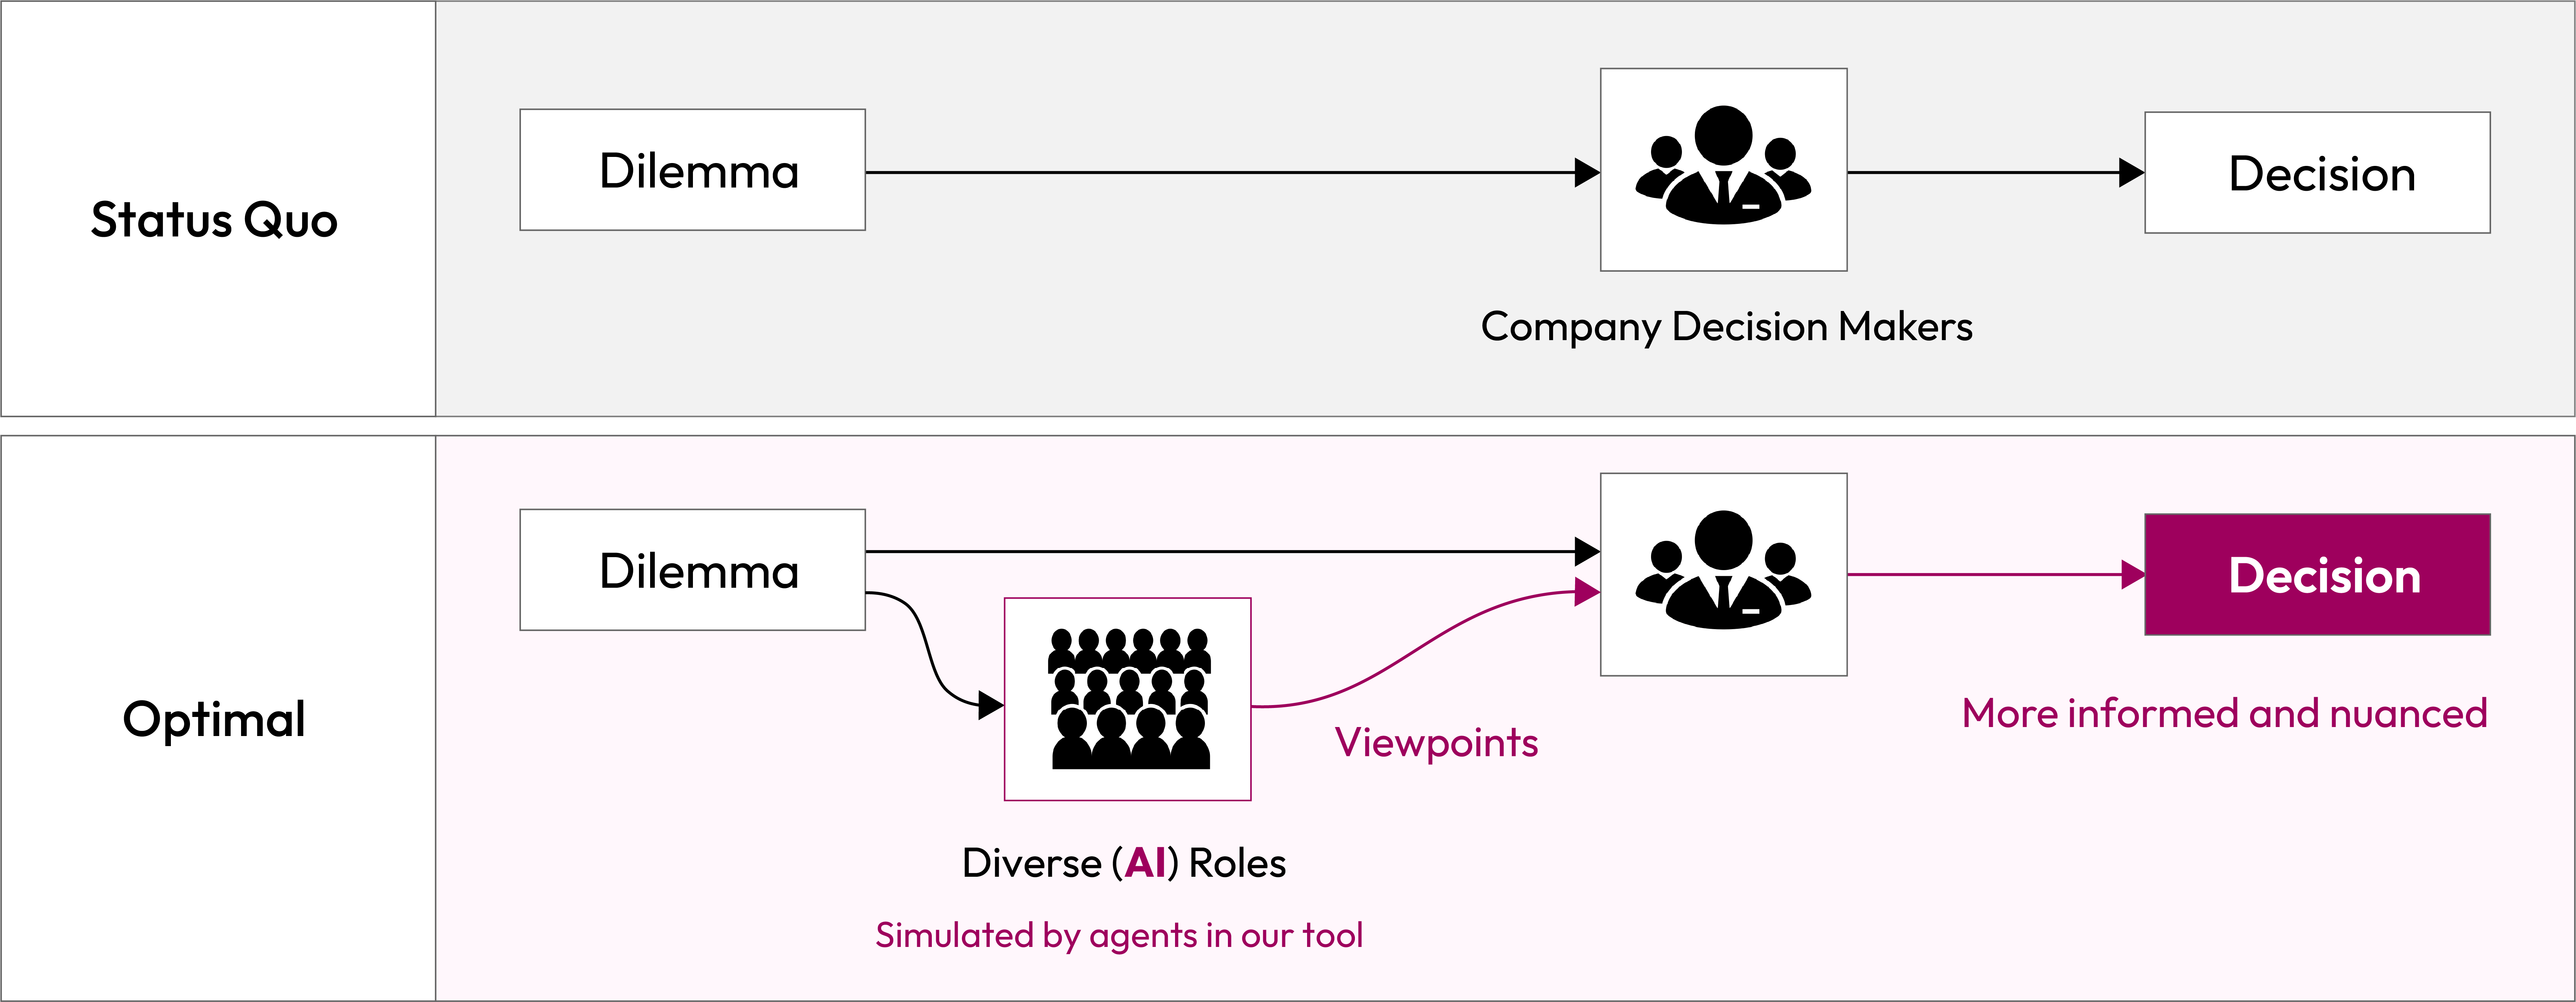
\includegraphics[width=\textwidth]{teaser}
  \caption{Overview of the Broken Morals project. Company decision-makers often address ethical dilemmas without structured access to diverse internal viewpoints (\textit{Status Quo}). In an optimal scenario, decisions are informed by multiple organizational roles, surfacing tensions and trade-offs that may otherwise go unexamined (\textit{Optimal}). In this study we propose a tool that approximates this ideal by simulating diverse role-based perspectives through artificial intelligence agents, supporting more reflective and nuanced moral reasoning.}
  \Description{Overview of the Broken Morals project}
  \label{fig:teaser}
\end{teaserfigure}

\received{2 June 2025}
\begin{comment}
\received[revised]{12 March 2009}
\received[accepted]{5 June 2009}
\end{comment}

%%
%% This command processes the author and affiliation and title
%% information and builds the first part of the formatted document.
\maketitle

\section{Related Work}

%Don’t review everything under the sun. Focus only on Problem Y.
%• Keep it to one page. If it drags on, you’re overcompensating.
%• End with this line: "To sum up, previous work has failed to address Y." Boom.
%• Can’t pinpoint a clear Y? Rewrite your Abstract/Intro/Related Work

In the current business landscape, complex corporate structures and pervasive technology have amplified concerns regarding organizational moral misalignment \cite{martinez}. This misalignment (a divergence between an organization's professed ethical values and the actual moral reasoning guiding its decisions) can foster ethical conflicts within the workplace. As Hyatt and Gruenglas \cite{hyatt} highlight, such conflicts "have profound effects on morals, code of conduct, and norms among stakeholders, which can ultimately undermine an organizational mission and its articulated values." High-profile cases like Volkswagen's emissions fraud \cite{ameen_2020} underscore how systemic failures can arise from unaddressed ethical weaknesses. These moral blind spots often originate not from deliberate misconduct but from structural and cognitive limitations within organizations \cite{sezer_etal_2015}.

To address such ethical challenges, scholarly work in business ethics has long investigated how ethical culture, principled leadership, and stakeholder governance influence organizational behavior \cite{donaldson_preston_1995}. However, despite these efforts, a growing body of research highlights key limitations. Past efforts to address these issues have often fallen short, partly because traditional top-down ethics reviews or approaches with limited stakeholder involvement frequently fail to capture the diversity of internal perspectives before critical decisions are made \cite{mitchell2020stakeholder, kujala}.

This gap becomes particularly evident with the increasing centrality of algorithmic systems in organizational decision-making. Despite this, the modeling of internal moral deliberation remains notably underexplored in computer science. Current computer science ethics research predominantly focuses on issues like fairness in machine learning \cite{mehrabi2022survey}, bias mitigation \cite{bianchi2023easily}, interpretability \cite{doshi-velez2017towards}, and responsible AI design principles \cite{leslieunderstanding, sandersonimplementing,sekrstai,sadek2025challenges}. While vital, these inquiries primarily address AI system outputs, not the organizational dialogues that inform their development \cite{madaio_etal_2020}. A notable gap remains in the application of computational methods to simulate internal ethical deliberations, especially those capturing conflicting viewpoints across diverse organizational roles \cite{herdel2024exploregen}. This stands in contrast to AI alignment research, which primarily aims to align agent objectives with broad human values \cite{gabrielartificial}. Consequently, a key challenge is to develop computational models capable of representing the complexity of moral pluralism within organizations \cite{sekrstai}.

To bridge this interdisciplinary gap, research is drawing from agent-based models \cite{gilbert_2022}. In Silico Sociology \cite{kozlowski_etal_2024} uses agents powered by Large Language Models (LLMs) to simulate complex social phenomena, offering a powerful lens to examine interactions across varied social roles and cultural norms. Agent-based models are increasingly used for simulating policy debates and moral scenarios. A notable advancement is the development of generative agent simulations involving over 1000 agents modeled on real individuals via qualitative interviews \cite{park_etal_2024_1000}. These simulations use LLMs to enable agents with specific personas to engage in structured social deliberations. Furthermore, systems like Plurals \cite{ashkinaze_etal_2025} are being developed to guide multi-agent deliberations, with LLMs potentially acting as moderators or structuring interactions. Such techniques allow researchers to identify consensus and disagreement, offering new insights into organizational ethical conflicts and providing scalable methods to evaluate ethical interventions \cite{rao_etal_2025_riskrags}. However, none of these techniques have been applied to the contex of organizational moral misalignment.

While traditional business ethics research has long focused on leadership, values, corporate responsibility, and governance, and computer science has prioritized algorithmic fairness, bias mitigation, and transparency, these domains have largely evolved in parallel. Few efforts have bridged these fields to examine how diverse internal perspectives shape ethical decisions in real-world decision-making.
To sum up, previous work has failed to efficiently address the inclusion of diverse perspectives in the context of company ethical decision-making.

By integrating insights from organizational behavior, responsible AI, and computational social science, we propose a new approach to support the formation of ethical decisions within complex institutions. Our work addresses this objective by introducing a multi-agent deliberation system to simulate internal moral reasoning across diverse organizational roles.


\section{Methods}
\label{sec:methods}

\begin{comment}
Here you explain how you’ve solved the problem
in our case

SITUATION: Problem X is very important because . . .
COMPLICATION: In tackling problem X, related work failed in doing Y
PROPOSAL: To partly tackle Y, we make N contributions [list of contributions]

X = organizational moral misalignment
Y = incorporating different perspectives

we solve the problem of incorporating different perspectives
so we explain how we did it
\end{comment}

To address the challenge of incorporating diverse organizational perspectives into ethical decision-making, we propose a software tool designed to support company decision-makers.
This section describes the design and operation of the tool we developed to simulate organizational moral reasoning using role-based AI agents.
We first explain the intended use of the tool and the type of input it receives from the user. We then describe how the system simulates the reasoning of three organizational roles using artificial intelligence agents. Finally, we detail how the tool generates a structured summary from these simulated perspectives and delivers it to the user.
Figure \ref{fig:impl} summarises the tool architecture.

\begin{figure}[h]
  \centering
  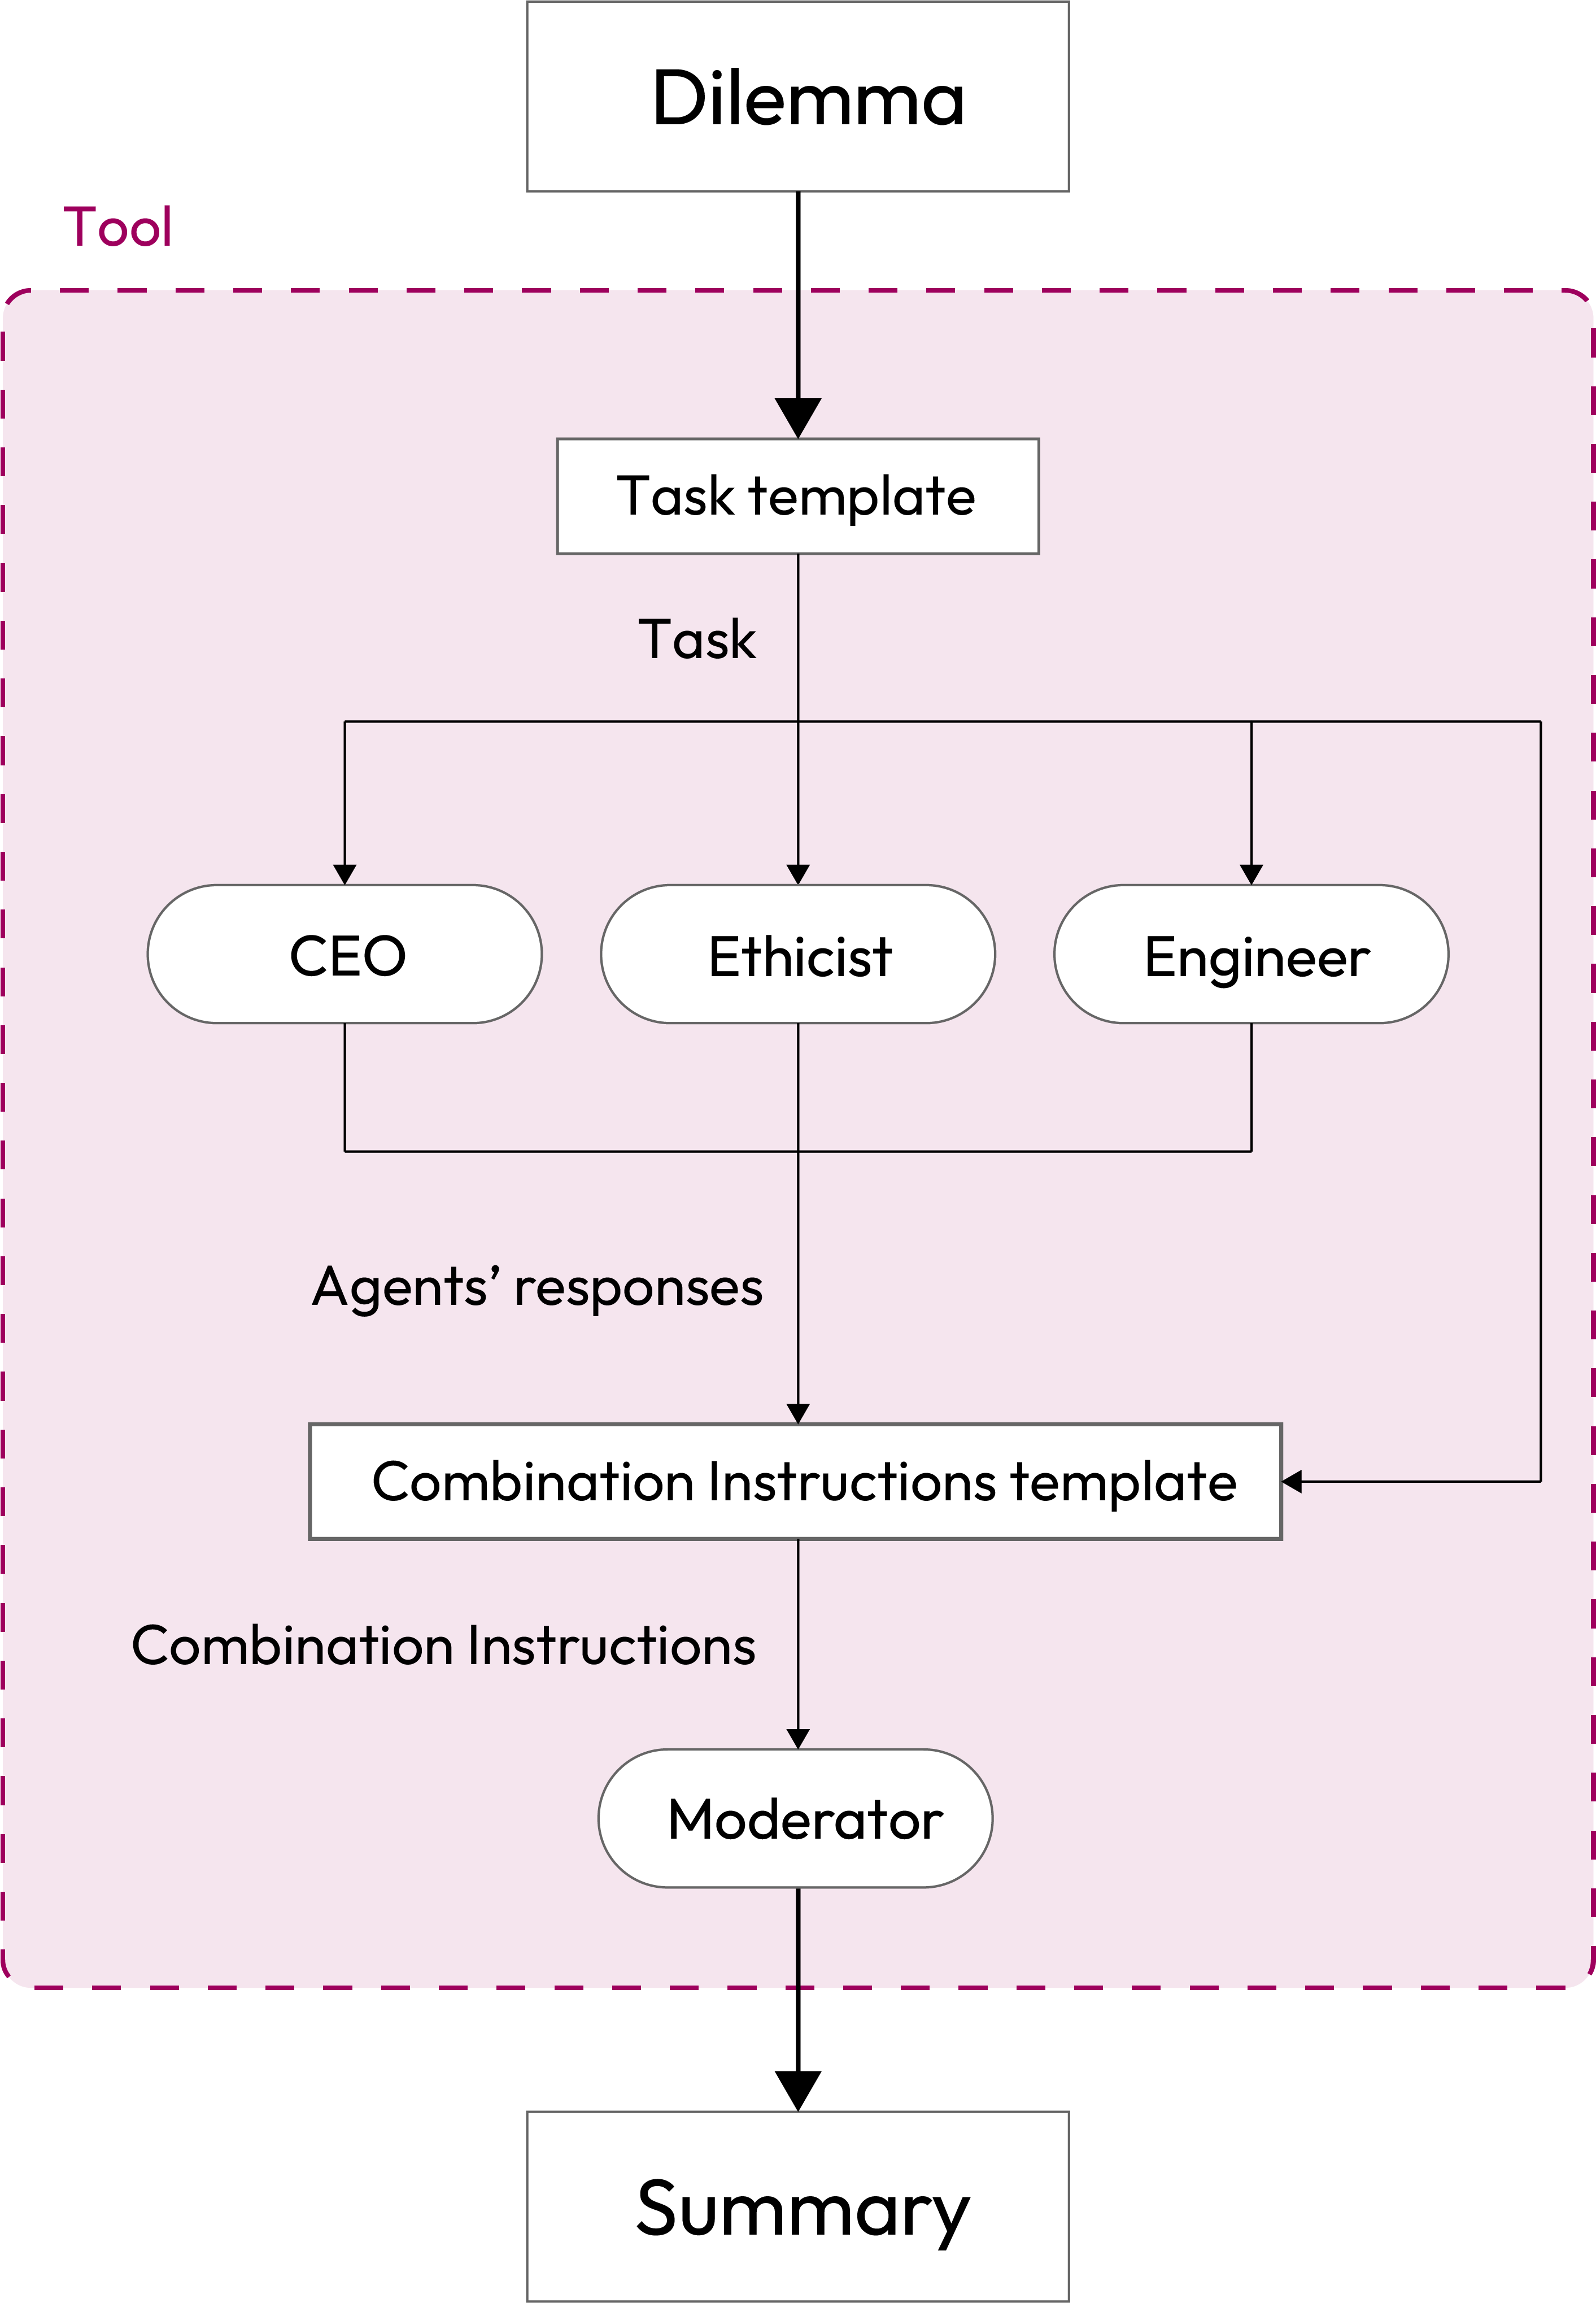
\includegraphics[width=\linewidth]{impl}
  \caption{Overview of the tool's architecture. The user provides a moral dilemma, which is embedded into a task template and submitted independently to three artificial intelligence agents representing the roles of CEO, ethicist, and engineer. Each agent responds based on a predefined persona prompt. The agents' responses are then passed to a moderator agent via a combination instructions template. The moderator analyzes the content and produces a structured summary highlighting agreement, disagreement, and suggested considerations for the user to cover in their answer.}
  \Description{Overview of our tool's architecture.}
  \label{fig:impl}
\end{figure}

\subsection{Tool Purpose and Use Context}

While ethical dilemmas in corporate contexts often involve conflicting viewpoints (such as operational feasibility, long-term impact, and normative values), real-world decision processes frequently lack mechanisms to systematically consider these different angles before a decision is made.
A software tool offers three primary advantages in this context. First, it provides structured access to a plurality of perspectives that may otherwise be inaccessible due to hierarchical, departmental, or cultural barriers. Second, it enables consistent and scalable reasoning support that can be applied to a wide range of cases without requiring additional personnel or meetings. Third, by relying on artificial intelligence agents prompted to emulate distinct organizational roles, the tool encourages users to reflect more critically on the trade-offs and value conflicts embedded in each dilemma.
The intended users are decision-makers in organizations: particularly those at the executive or senior management level, who are often required to resolve complex ethical scenarios quickly, under uncertainty, and without comprehensive stakeholder input. Our tool aims to enrich this decision process by making invisible perspectives explicit, in a structured and neutral form.

\subsection{Dilemma Input}

The user begins by inputting a moral dilemma into the tool.
In our context, a dilemma is defined as a scenario describing a realistic organizational situation that involves an ethically relevant conflict. A dilemma includes a brief narrative containing background information (the description of a scenario, including the roles of the stakeholders involved, the context in which the decision must be made, and any relevant constraints) followed by one or more open-ended questions requiring the user to take a position or justify a course of action.
By formulating the dilemmas in this way, we ensure that the tool operates on rich, ambiguous inputs that reflect the types of challenges decision-makers face in real-world contexts.

\subsection{Role-based Agents}

\paragraph{Persona Prompts}{
  Once the dilemma is submitted, the tool initiates an internal simulation involving three artificial intelligence agents, powered by large language models (LLMs). Each agent is assigned a fixed organizational role: a chief executive officer, an engineer, and an ethicist. These roles were selected to reflect three core domains of organizational reasoning: strategic authority, technical feasibility, and moral evaluation.
  To ensure that each role-based agent reliably reflects its assigned organizational role, we design tailored prompts that define the agent's responsibilities, values, and communication style. Each prompt specifies the agent's professional identity within a fictional mid-sized company and outlines the reasoning strategies it should apply when responding to the dilemma.
  These role-specific prompts (referred to as \textit{personas}) are not simply character sketches; they are designed to elicit structurally distinct forms of reasoning that mirror real-world organizational tensions.
  The CEO agent (Prompt \ref{prompt:ceo}) is instructed to prioritize long-term organizational success, brand reputation, and strategic decision-making, with a focus on risk-benefit trade-offs and pragmatic leadership. The engineer agent (Prompt \ref{prompt:engineer}) emphasizes feasibility, technical integrity, operational constraints, and potential implementation risks. The ethicist agent (Prompt \ref{prompt:ethicist}) centers its reasoning on moral principles, stakeholder rights, and social responsibility, often challenging decisions that may appear effective but raise ethical concerns.
}

\paragraph{Task}{
  The simulation starts by instantiating the three role-based agents and dispatching a common task to each of them individually. To construct the task, we embed the user-provided dilemma into a common task template (Prompt \ref{prompt:task}). This template instructs an agent to read the dilemma and respond in approximately 300 words, providing their reasoning, thoughts, and opinions. Each agent receives this same structured task, but interprets and responds to it according to the role-specific instructions defined in their \textit{persona} prompt.
}

\paragraph{Topology}{
  Rather than engaging in freeform debate, the agents operate within a standardized discussion topology. The agents respond independently, without direct interaction with one another. This design choice reflects our goal of faithfully simulating distinct organizational viewpoints without introducing conversational dynamics such as persuasion, alignment, or social conformity that may occur in natural group discussions. This \textit{Ensemble} structure ensures clarity and prevents conversational drift, allowing each agent to contribute a distinct, coherent viewpoint. This topology is not designed to reach consensus, but rather to expose areas of convergence and divergence in how each role interprets the dilemma.
}

\subsection{Summary Output}
\label{sec:summary}

\paragraph{Moderator Agent}{
  Once the three role agents have expressed their positions, a fourth agent, the Moderator, is activated using a separate instruction set: the \textit{combination instructions} (Prompt \ref{prompt:combination}). This prompt defines the moderator's objective as supporting a human decision-maker by analyzing and summarizing the agents' individual outputs in a structured, accessible format. The moderator is explicitly instructed to identify and present the core tensions raised in the responses, areas of agreement and disagreement among the agents, and a list of practical considerations that the user should address in their own justification. The moderator's tone is constrained to be neutral, direct, and free of technical or philosophical jargon, to ensure accessibility and minimize framing bias.
}

\paragraph{Summary Structure}
The moderator thus produces a summary that is composed of three parts: (1) a list of points on which the agents agreed, providing a sense of organizational alignment; (2) a list of disagreement areas and competitive priorities, revealing underlying tensions or conflicting viewpoints between roles; (3) a set of practical questions or considerations that the user is encouraged to reflect on when making their own decision.
This design emphasizes cognitive support over persuasive framing, aiming to augment the user's moral reflection without biasing the outcome.
The purpose of this output is not to recommend a specific course of action, but to broaden the user's moral reasoning by foregrounding perspectives they may overlook. By surfacing both consensus and conflict among roles that typically shape corporate decision-making, the tool helps users critically examine their own intuitions, mitigate personal blind spots, and produce more structured, well-reasoned responses.


\section{Evaluation}

The goal of our tool is to support company decision-makers in generating more reflective and ethically grounded responses to business dilemmas than they would produce using unaided reasoning.

To ascertain whether our tool meets this goal, our evaluation aims to answer the following questions:
(a) Effectiveness: Do participants who use the tool produce higher-quality justifications compared to those who do not?
(b) Effort: Does the tool significantly increase the time required to answer a dilemma?
(c) Perceived Usefulness: Do users perceive the tool's output as helpful in supporting their reasoning?

To measure these aspects, we conducted a controlled user study with 50 senior professionals from the technology sector. Participants were asked to respond to business ethics dilemmas, with half assigned to a treatment group receiving the tools output, and half to a control group completing the task unaided. Responses were evaluated using a custom six-dimensional rubric. We also collected response time data and post-task feedback.

This section describes the tool implementation and the evaluation setup, including dilemma selection, participant recruitment, scoring rubric design and data analysis pipeline. We then report the results and discuss their implications.

\subsection{Tool Implementation}

We implemented the proposed tool (described in Section \ref{sec:methods}, Figure \ref{fig:impl}) using the Plurals framework \cite{ashkinaze2025pluralsguidingllmssimulated}, a Python library that orchestrates LLM agents to simulate structured deliberations.
Plurals simplifies the definition of role-based agents, discussion topologies, and moderation logic, and provides an abstraction layer over different LLM backends.
All agents and the moderator in our setup used GPT-4.1 as the underlying language model.
For the moderator agent, we adopted the default moderator persona provided by Plurals: an expert impartial observer responsible for overseeing the common task.
To reflect our tool definition, we selected the \textit{Ensemble} topology (among the topologies supported by Plurals), and set the number of cycles to one, meaning each agent contributes a single, uninterrupted response to the dilemma before the summary is generated.
Executing a full run of the system on a single dilemma requires four API calls to OpenAI: three for the role agents and one for the moderator. Using the set of dilemmas described in Section \ref{sec:dilemmas}, each complete simulation averaged $5k$ tokens total ($4k$ input tokens, $1k$ output tokens) across all calls.


\subsection{Dilemma Set and Tool Summaries}
\label{sec:selected_dilemmas}

This section reports the dilemmas we selected in Section \ref{sec:dilemmas}, their moral classification scores (Table \ref{tab:foundation-scores}), the generated tool's summaries.
The final question(s) of each dilemma have been slightly altered with respect to the cited version to ensure participants would produce more articulated responses instead of short ones. For dilemmas that already had a set of reflection points provided by the author, we remove them to simulate a realistic scenario in which users has to produce those reflection themselves, or with the help of our tool.
Each summary was presented in the Treatment group form after the dilemma description and question(s) with the following introduction: "\textit{Here is a summary of a debate between different figures (a CEO, an engineer, and an ethicist) regarding this dilemma.}".

\begin{table*}[t]
  \centering
  \caption{Moral classification scores for the selected dilemmas (rounded to two decimal digits). Each moral foundation can be present in the form of \textit{virtue} or \textit{vice}: capital letters represent the virtue label, lowercase letters represent the vice. Legend: Care (c), Fairness (f), Loyalty (l), Authority (a), Sanctity (s).}
  \begin{tabular}{lcccccccccc}
    \toprule
    \textbf{Dilemma} & \textbf{C} & \textbf{c} & \textbf{F} & \textbf{f} & \textbf{L} & \textbf{l} & \textbf{A} & \textbf{a} & \textbf{S} & \textbf{s} \\
    \midrule
    \ref{sec:facebook} & 0.99 & 0.95 & 0.99 & 0.23 & 0.98 & 0.24 & 0.97 & 0.49 & 0.36 & 0.19 \\
    \ref{sec:apple} & 0.91 & 0.99 & 0.01 & 0.06 & 0.01 & 0.05 & 0.99 & 0.49 & 0.01 & 0.05 \\
    \ref{sec:mm} & 0.98 & 0.00 & 0.98 & 0.01 & 0.98 & 0.01 & 0.95 & 0.03 & 0.02 & 0.01 \\
    \ref{sec:ut} & 0.99 & 0.01 & 0.03 & 0.93 & 0.99 & 0.30 & 0.99 & 0.11 & 0.76 & 0.89 \\
    \ref{sec:ben} & 0.99 & 0.72 & 0.02 & 0.37 & 0.99 & 0.14 & 0.70 & 0.40 & 0.35 & 0.06 \\
    \bottomrule
  \end{tabular}
  \label{tab:foundation-scores}
\end{table*}

\subsubsection{Facebook and our Fake News Problem \cite{1_fb}}
\label{sec:facebook}

\begin{quote}
  The 2016 election season generated many headlines, some of which are notable for being blatantly false. Fake news ranged from, "the Pope endorsed Donald Trump" all the way to "Hilary Clinton is running a child sex ring out of a pizza shop." Did "fake news" influence the outcome of the 2016 US Presidential election? While the answer is unclear, one thing is certain. The rise of fake news has reached unprecedented levels and has raised serious concerns about how citizens receive their news and form opinions. The increase in fake news has several sources. Social media platforms like Facebook gave these stories the same visibility as news publications, such as those from the New York Times or Wall Street Journal. Moreover, these posts often had higher engagement rates (comments and reactions) resulting in them receiving even higher visibility and prevalence in users' news feeds. Facebook CEO Mark Zuckerberg initially downplayed the problem, calling it a "pretty crazy idea" that fake news on Facebook influenced the election. Zuckerberg has since begun to address the fake news issue, but warns, "We must proceed very carefully... and must be extremely cautious about becoming arbiters of truth ourselves." The Society of Professional Journalists has a code of ethics with four principles: seek truth and report it; minimize harm; act independently; and be accountable and transparent. But the transition to online platforms has fundamentally changed journalism. Google and Facebook control 80 percent of ad revenues; the same revenue source that news publishers depend on. Moreover, more than 40 percent of people now get their news from social media networks - making Facebook a de facto middleman in people's intake of news. Facebook is taking the problem seriously, albeit with a great deal of caution. They have introduced efforts to help users spot fake news and inject indicators of trust (disputed tags) into their posts in partnership with a few institutions. They have also banned fake news sites from advertising on the network.
\end{quote}

\paragraph{Questions}{
  Does Facebook have an obligation to address the fake news problem? If so, what should be done about it?
}

\paragraph{Tool's Summary}{
  \begin{description}
    \item[Core Tension in the Debate] The central tension is between Facebook's responsibility to limit the spread of fake news and the challenges of doing so in a way that avoids censorship, protects free speech, and maintains trust. There is also a balance to strike between Facebook acting as a neutral platform and its real role as a powerful influence over public opinion.
    \item[Points of Agreement] All perspectives agree Facebook has an obligation to address fake news due to its scale and influence.
      There is agreement that doing nothing risks harm to individuals, society, and Facebook's reputation and business.
      All recognize that transparency and user empowerment are important; users should understand how news is vetted and have tools to judge credibility.
      Each supports partnerships with independent fact-checkers and increased media literacy efforts.
      Limiting the reach and monetization of fake news is seen by all as sensible and achievable.
    \item[Areas of Disagreement] The CEO's perspective emphasizes business risks, brand trust, and stakeholder engagement, focusing on sustainable growth and regulatory concerns.
      The ethicist urges stronger action based on moral duties to society and individual users, prioritizing truth and autonomy, and calls for even greater transparency and independent ethical oversight.
      The engineer accepts responsibility but highlights the technical complexity and risk of over-enforcement, warning that overreach could lead to accusations of censorship and implementation mistakes.
    \item[Practical Points to Consider in Your Answer]{
        \hfill
        \begin{enumerate}[label=(\alph*)]
          \item How far should Facebook go in moderating content without overstepping into censorship?
          \item What level of transparency is necessary to build user trust and credibility?
          \item How can Facebook ensure its actions are effective but also respectful of diverse viewpoints and global contexts?
          \item What checks and balances (like appeals and oversight) are needed to handle errors and criticism fairly?
          \item What is the right mix of technology and human judgment in addressing misinformation at scale?
          \item How can long-term strategies for user education and media literacy be integrated.
        \end{enumerate}
      }
  \end{description}
}

\subsubsection{Apple \textit{vs.} FBI Case Study \cite{2_af}}
\label{sec:apple}

\begin{quote}
  In the wake of the December 2015 terrorist attack in San Bernardino, attention turned to the perpetrator's iPhone. A federal judge asked Apple, maker of the iPhone, to provide "reasonable technical assistance" to the FBI in accessing the information on the phone with that hope of discovering additional threats to national security. Apple provided the FBI with data it had in their possession and sent Apple engineers to advise the FBI, but refused to comply with the court order to bypass the phone's security measures: specifically the 4-digit login code and a feature that erases all data after ten incorrect attempts. The FBI argued that the bypass could only be used for this phone, this one time. The agency also cited national security concerns, given the phone may lead to better understanding the attack and preventing further incidents. Apple CEO Tim Cook issued a public letter reiterating Apple's refusal to cooperate. Cook advocated for the benefits of encryption in society to keep personal information safe. He stated that creating the backdoor entry into the iPhone would be akin to creating a master key capable of accessing the tens of millions of iPhones in the U.S. alone. Cook also had concerns that the FBI was outstepping its bounds - by using the court system to expand its authority - and believed the case should be settled after public debate and legislative action through Congress instead. Public opinion polls on the issue were split. A number of major tech firms filed amicus briefs in support of Apple. The White House and Bill Gates stood behind the FBI. In anticlimactic fashion, the FBI withdrew its request a day before the hearing, claiming it no longer needed Apple's help to assess the phone. It is speculated that an Israeli tech firm, Cellebrite, helped the FBI gain assess.
\end{quote}

\paragraph{Questions}{
  Was Apple wrong for not complying with the FBI's request? If so, why? If not, why not?
}

\paragraph{Tool's Summary}{
  \begin{description}
    \item[Core Tension in the Debate] The central conflict is between national security and individual privacy. The FBI wanted access to the iPhone to possibly prevent further threats, while Apple believed creating a security bypass would endanger the privacy and security of all users. There's also a tension between quick action in a crisis and the need for broad, democratic debate before setting far-reaching precedents.
    \item[Points of Agreement] All roles agree that law enforcement has a legitimate concern and reason for wanting access to the device.
      Each viewpoint acknowledges that creating a backdoor or bypass tool could have broader implications beyond this single case.
      There is consensus that Apple cooperated as much as it could by providing data already in its possession.
      All parties stress the importance of trust—between the company and its users, and between the public and institutions.
    \item[Areas of Disagreement] The CEO is most focused on protecting the company's reputation, market value, and customer loyalty.
      The engineer highlights the technical impossibility of a secure “one-time” bypass and the risk of unintended spread if such a tool were developed.
      The ethicist emphasizes the broader ethical responsibility to protect user rights, and the importance of open, democratic processes over judicial expedience.
    \item[Practical Points to Consider in Your Answer]{
        \hfill
        \begin{enumerate}[label=(\alph*)]
          \item Should companies be compelled to weaken their product security for law enforcement, even in extreme cases?
          \item What are the long-term consequences of creating tools that can bypass security for any single case?
          \item How should society balance immediate security demands with the risk to broader privacy and civil liberties?
          \item Should issues with wide public impact be resolved by courts or through legislative, democratic means?
          \item What precedent would compliance set for future government or international demands for access?
        \end{enumerate}
      }
  \end{description}
}

\subsubsection{Misinterpretation Mishap \cite{3_mm}}
\label{sec:mm}

\begin{quote}
  Tony is a project leader at a company frequently subcontracted to produce code for various U.S. government entities and affiliates. Traditionally, code that was developed for one federal department could be reused for another if approval was obtained by the former. One day, Tony's company was contacted by a privately-owned commercial corporation, FlyHigh, to create code for an avionics-related image processing effort. Since the code requested was almost identical to one used for a past project, Tony's team decided to, once approval had been obtained from the government, reuse the code. After permission was granted through email, however, Tony realized the approving party, a law agency that was contracted by the government, lacked complete understanding of who would benefit from the reused code. Tony wanted to contact the government directly to ensure it had been informed of all vital aspects of the contract, but realized doing so could mean having the initial approval revoked, having to re-code the requested code, and increasing the contract bid up to two million dollars.
\end{quote}

\paragraph{Questions}{
  Understanding the contract between his company and FlyHigh was on the line, should Tony move forward with clarifying the situation to the appropriate party? Why? If so, how?
}

\paragraph{Tool's Summary}{
  \begin{description}
    \item[Core Tension in the Debate] The central dilemma is whether Tony should clarify code reuse approval directly with the appropriate government authority—even if it risks delaying the project, increasing costs, or losing a valuable contract. The trade-off is between short-term business gain and the longer-term risks of legal trouble, reputational harm, and ethical lapses if the approval obtained isn't fully informed.
    \item[Points of Agreement] All roles agree Tony should clarify the situation with the proper government entity.
      They identify that the approval already given could be based on incomplete information.
      Each perspective sees long-term legal, reputational, and ethical risks in proceeding without proper, explicit government consent.
      All would notify FlyHigh about the potential delays or additional costs, to be transparent with the client.
      They recognize the importance of commitment to integrity and trust in maintaining business relationships.
    \item[Areas of Disagreement] The CEO puts a strong emphasis on the company's reputation, risk management, and long-term business viability.
      The engineer/ethicist focuses more on professional and ethical duties: transparency, responsible use of public resources, and respect for the original owner's intent.
      There may be varying tolerance for short-term business pain, with some more willing to accept potential financial losses for the sake of compliance and ethics.
    \item[Practical Points to Consider in Your Answer]{
        \hfill
        \begin{enumerate}[label=(\alph*)]
          \item Who is authorized to give true, informed approval for code reuse in this context?
          \item What are the potential consequences (legal, financial, reputational) of proceeding without clarification?
          \item How should Tony communicate with the government and FlyHigh to be transparent about the approval process and its impact on timelines or costs?
          \item What steps can be taken to ensure full understanding and documentation if similar situations arise in the future?
        \end{enumerate}
      }
  \end{description}
}

\subsubsection{Unchartered Territory \cite{4_ut}}
\label{sec:ut}

\begin{quote}
  David Johnson holds a major leadership position within an established biotechnology firm. The firm has successfully pursued wildly innovative research utilizing DNA that has pushed the boundaries of science. Many potential clients - from universities and medical centers to private institutions - expressed a strong interest in the company's technology. Knowing that this technology was both powerful and relatively unregulated by the government, both Johnson and the company were keen to monitor who they sold their products to. The company's solution was to investigate potential clients and only sell to those who demonstrated "bona fide use", i.e. a legitimate use that would be carried out in good faith. However, determining what was and was not bona fide use proved to be tricky. Some researchers wanted to use the technology to investigate the genes of specific ethnic groups in order to understand common genetic diseases within that group. While this particular project was intended to benefit people, the company was concerned about how that information could potentially be used in the future, not to mention the company's culpability for that use given that its technology was used in the research. The company was concerned that the kind of information the potential customer would have access to could be used to discriminate against people with certain genetic markers, particularly by insurance companies looking to increase rates for clients at a higher risk for illness. At the same time, the investors of the biotech firm expect a return, given the high costs of research and development as well as the amount of risk they took on funding the project.
\end{quote}

\paragraph{Questions}{
  Does the firm have an obligation to self-regulate their product? Are their "bona-fide use" standards sufficient?
}

\paragraph{Tool's Summary}{
  \begin{description}
    \item[Core Tension in the Debate] The main tension is between maximizing business success—including satisfying investors and pursuing innovation—and ensuring ethical responsibility in using potentially dangerous biotechnology. The dilemma centers on how far a company must go to prevent harm from even unintended uses of its product, particularly when regulations are not yet robust.
    \item[Points of Agreement] All roles agree the company has a clear obligation to self-regulate, given the potential for misuse and lack of government oversight.
      They concur that existing “bona fide use” standards are not strong enough, being too subjective and open to interpretation.
      Each acknowledges that failure to regulate could lead to reputational, legal, and financial risks, undermining both ethics and business stability in the long run.
    \item[Areas of Disagreement] The CEO places emphasis on balancing ethical duties with investor expectations, highlighting reputation and business sustainability. Their proposed actions focus on risk mitigation for both business and ethics.
      The engineer is especially concerned about process: they call for detailed, documented frameworks (like clear vetting criteria, ongoing monitoring, and cross-functional review), suggesting the standards must be operationally robust and repeatable. The ethicist pushes for even stronger measures such as independent oversight, contractual restrictions, and refusing sales if risks cannot be mitigated, consistently putting ethical concerns over profits.
    \item[Practical Points to Consider in Your Answer]{
        \hfill
        \begin{enumerate}[label=(\alph*)]
          \item How will the company define and operationalize “bona fide use” in a way that is clear, consistent, and resistant to abuse?
          \item What specific processes or checks should be in place to vet and monitor customers and research projects?
          \item How far should the company go in refusing sales or severing relationships if future misuse is possible but uncertain?
          \item What balance should be struck between meeting investor expectations and fulfilling ethical obligations when they conflict?
          \item How can long-term risks (reputational, legal, ethical) be weighed against short-term business gains?
        \end{enumerate}
      }
  \end{description}
}

\subsubsection{Balancing Culture and Ethics \cite{5_ben}}
\label{sec:ben}

\begin{quote}
  Ben is a dedicated manager at a prominent multinational company, where he manages teams spread across different countries that ultimately report back to him in California. Ben finds a great deal of fulfillment in his work, particularly when he has the opportunity to travel and visit his team leads around the world. Ben made it a point to immerse himself in the local culture during his business travels, dedicating an extra day or two to learn about the culture before heading into his company's office or factory in whatever location he was at. On one trip, Ben traveled to Chennai, India, to visit JP, a lead manager in the local operation. Ben asked JP to spend the day with him exploring the area and its traditions, and JP graciously agreed and took Ben on an eye-opening excursion to a nearby village that, like many in rural India, was poor. Ben noticed JP's close connections with the villagers. JP, an esteemed member of the Brahmin caste and an elder at the Hindu temple, was highly respected and considered a leader in the community. Ben was grateful for the warm welcome extended to him by the villagers and appreciated the effort JP put into arranging this visit. But Ben also found himself in an uncomfortable spot. JP wanted to take Ben to this particular village not only because he knew the people well, but also because a local Chennai clothing company had recently established a business here and he thought Ben would be interested in this new development. The company had adopted a business model that involved renting looms to families in the village, which enabled them to produce cloth materials and fulfill orders from the company. While the families earned money for the piece work, they also had to pay the rent for the looms. As Ben observed the process, he couldn't help but notice children as young as ten working at the looms. When visiting one family, Ben and JP met with the parents who told them how this local business was really helping their family. And, as they said that, their two children sat nearby working at the looms. Ben was cut to the core. He had read about the dangers of child labor and in particular about the way that work on looms can be especially harmful (and how children due to their better eyesight and ability to see subtle distinctions in color are in demand to work on looms). These conditions pose significant risks to children, especially in terms of the potential hazard of diminishing their eyesight and its impact on their overall well-being. It pained him to see these children working while he envisioned his own eight and 11 year-old kids back home (the children in Chennai were about the same age) engaging in such laborious, risky tasks. He would never let his own kids do it. Then again, he thought: I'm not dealing with the circumstances these parents are dealing with. Ben was aware of how JP spoke very positively about the village and the additional income the children's labor provided for the families. It was also clear that the children's parents didn't object and that the whole village appeared to be on board with this income-producing project. As Ben's visit to the village came to an end, some of the villagers, including JP, eagerly asked him to share with them his thoughts on the new business development in the village.
\end{quote}

\paragraph{Questions}{
  Should he approve of it? Why? What should Ben say?
}

\paragraph{Tool's Summary}{

  \begin{description}
    \item[Core Tension in the Debate]  The main issue is whether the economic benefits to families in the village justify allowing children to work in potentially harmful conditions. There is a conflict between respecting the community's desire for income and opportunity, and upholding the ethical imperative to protect children from exploitation and long-term harm.
    \item[Points of Agreement]  Everyone agrees the villagers' hospitality and local leadership deserve respect. There is consensus that the business brings much-needed income to struggling families. All roles recognize that child labor, especially in hazardous settings, presents serious risks to children's health, safety, and development. Each participant believes the conversation must be approached with sensitivity and honesty, avoiding blame or judgment.
    \item[Areas of Disagreement] There may be differences in how forcefully to express opposition to child labor. The ethicist takes a firm stance against it as a universal wrong, while the engineer and CEO might focus more on balancing cultural sensitivity with the need for reform. The CEO is more concerned about corporate responsibility and reputation, insisting the company should not be linked to harmful labor practices, while the engineer analyzes the operational side (financial risk and youth impact). They differ on the role of cultural relativism: the ethicist and CEO lean towards universal standards, while the engineer emphasizes collaboration and understanding local context before taking action.
    \item[Practical Points to Consider in Your Answer]{
        \hfill
        \begin{enumerate}[label=(\alph*)]
          \item How can Ben express his concerns honestly and respectfully, recognizing the villagers' realities?
          \item Should Ben recommend the business model as it is, suggest modifications, or oppose it outright due to the child labor issue?
          \item How might he encourage solutions that keep children safe and in school, while still supporting the village's economic needs?
          \item What responsibility does Ben or the company have to advocate for universal ethical standards, even in another culture?
          \item How can long-term harm to children be prevented without undermining the community's autonomy and trust?
        \end{enumerate}
      }
  \end{description}
}


\subsection{Participants Recruitment}

To evaluate the effectiveness of our tool with a relevant population, we recruited participants through the Prolific platform, targeting professionals in the technology sector with decision-making responsibilities in high-stakes organizational contexts.
We applied several screening criteria to ensure both relevance and quality of the responses. Eligible participants respected the following criteria:
(1) currently residing in an english speaking
(2) holding a senior work role
(3) having a 100\% approval rate on previous Prolific submissions
The exact screeners we used can be found in Description \ref{desc:screeners}.
These screeners were designed to increase the likelihood of finding fluent English speakers to reduce language-related confounds, and ensure that participants would possess both the soft skills and practical experience necessary to produce grounded, high-quality justifications when responding to complex moral dilemmas.
The compensation was set at £9 per hour, aligning with Prolific's recommended fair pay rate for tasks of this type.
Participants were shown a short study description prior to consenting, emphasizing that the task involved reading a scenario and providing a written answer, and asking them explicitly not to use AI tools in order to preserve the integrity of the human reasoning evaluation. The full participant-facing prompt is available in Description \ref{desc:study}.

\subsection{Participant Groups and Tasks}
control, treatment, form format, pay, time, task, questionnaires


\subsubsection{Six-Dimensional Rubric}
\label{sec:rubric}

To compare the quality of responses across the control and treatment groups, we required a consistent and meaningful evaluation method. Given the complexity and subjectivity of moral reasoning, we could not rely on simple correctness metrics or automated scoring. Instead, we developed a human evaluation rubric designed to break down each response into discrete, assessable dimensions, reflecting the depth, clarity, and practical quality of ethical reasoning.

We began by reviewing relevant literature in areas including argumentation theory, ethical decision-making, dialogue systems, and communication studies. From this review, we identified six key dimensions that collectively capture the qualities we aimed to evaluate. Each dimension is supported by prior research and was selected to align with the goals of our study.
The following list contains each dimension in our rubric, the questions an evaluator ought to answer in order to assigning a score to a participant's response, and the reference onto which the dimension is based:

\begin{description}
  \item[Clarity] \textit{Does the response express its ideas clearly? Is the reasoning easy to follow and well-organized?}
    Based on \citep{mctear2005spoken}, which highlights the importance of structure and readability in effective communication.
  \item[Relevance] \textit{Does the response stay focused on the moral dilemma? Are the points made directly connected to the question?}
    Informed by \citet{habernal2016argument}, which shows that content relevance strengthens argument quality.
  \item[Persuasiveness] \textit{Is the argument convincing? Does it use logic, appropriate tone, and structure to support its claims?}
    Drawn from \citet{johnson2006logical}, which emphasize the role of logical and well-structured reasoning in persuasion.
  \item[Concern for Long-Term Consequences] \textit{Does the response consider future or societal effects of the proposed action?}
    Inspired by the Impact Assessment Card \citep{impactassessment2018cscw}, which promotes ethical foresight.
  \item[Practical Usefulness] \textit{Is the proposed solution realistic? Could it work in practice?}
    Based on \citet{bazerman2012judgment}, who stress the importance of actionable and realistic decision-making.
  \item[Awareness of Context] \textit{Does the response take into account the social, cultural, or situational context of the dilemma?}
    Also from the Impact Assessment Card \citep{impactassessment2018cscw}, which encourages attention to contextual factors in ethical reasoning.
\end{description}

Each dimension was scored on a 5-point Likert scale, from 1 ("very low") to 5 ("very high"). The rubric provided the conceptual framework for qualitative evaluation, while the scoring process itself is described in the next section.


\subsection{Scoring the Answers}
\label{sec:scoring}

Evaluating open-ended ethical responses is inherently challenging, particularly when the goal is to compare two groups in a fair and unbiased manner. To ensure both reliability and impartiality, we followed a structured scoring process grounded in the evaluation rubric described in Section \ref{sec:rubric}.

We began by generating three identical scoring files, one for each rater. Each file included an \texttt{AnswerID} (unique for each participant) and the six rubric dimensions, but excluded any information about the group assignment (control or treatment). This ensured that the evaluation process was conducted blind to condition.

Each rater independently scored every response using the 5-point Likert scale across all six dimensions. After all ratings were collected, we reattached the group labels and computed inter-rater reliability using Fleiss' Kappa, separately for the control group, the treatment group, and both groups. Our target threshold was a Kappa value of 0.6 or higher, a standard benchmark for substantial agreement.

Initial agreement fell short of this threshold on some dimensions. To address this, we held a calibration session in which raters reviewed discrepant cases (still blind to condition), discussed interpretive inconsistencies, and refined their understanding of the rubric. After this reconciliation process, we rescored selected responses as needed and achieved the inter-rater agreement levels reported in Table \ref{tab:kappa}.

\begin{table}[H]
  \centering
  \caption{Fleiss' Kappa Scores by Dimension and Group}
  \resizebox{0.40\textwidth}{!}{%
    \begin{tabular}{lccc}
      \toprule
      \textbf{Dimension} & \textbf{Control} & \textbf{Treatment} & \textbf{Both} \\
      \midrule
      Clarity & 0.638 & 0.631 & 0.645 \\
      Relevance & 0.627 & 0.794 & 0.733 \\
      Persuasiveness & 0.696 & 0.625 & 0.681 \\
      Concern for Long--Term Consequences & 0.602 & 0.681 & 0.671 \\
      Practical Usefulness & 0.595 & 0.709 & 0.683 \\
      Awareness of Context & 0.592 & 0.672 & 0.667 \\
      \bottomrule
    \end{tabular}
  }
  \label{tab:kappa}
\end{table}

With these agreement levels in place, we computed the mean score across raters for each dimension, per response. The resulting dataset contained the following fields: \texttt{AnswerID}, \texttt{DilemmaID}, \texttt{Group}, followed by the six averaged rubric scores. This dataset served as the foundation for our statistical analysis, described in the next section.



\subsection{Results}

TODO PYRAMID INTRO

The tool-assisted Treatment group consistently outperformed the Control group across all six evaluative dimensions. These improvements ranged from medium to large effect sizes and remained statistically robust after controlling for non-normal data distributions and multiple hypothesis testing. Figure \ref{fig:distributions} shows the distributions of rating scores along each dimension of the evaluation rubric for both Control and Treatment groups. This section reports the exact statistical tests conducted on the evaluation dataset constructed in Section \ref{sec:scoring}.

\subsubsection*{Statistical Approach}

We tested for normality using the Shapiro-Wilk test and found violations in at least one group for each dimension. For example, in the \textsc{Clarity} dimension, the Control group yielded $W = 0.8817$, $p = 0.0075$ (significant at $\alpha = 0.05$), indicating departure from normality. Similar violations occurred across other dimensions (e.g., \textsc{Relevance} in the Treatment group: $W = 0.8839$, $p = 0.0083$). Given these violations and the ordinal nature of Likert data, we used non-parametric Mann-Whitney U tests (one-tailed) for all group comparisons.
The rank-biserial correlation ($r$) was chosen as the most appropriate effect size for the Mann-Whitney U, where $r = 0.1$, $0.3$, and $0.5$ represent small, medium, and large effects, respectively.

\subsubsection*{Primary Findings}

All six dimensions showed statistically significant differences favoring the Treatment group. Median scores were higher in every case, with Mann-Whitney U tests indicating reliable group differences. Effect sizes were quantified using rank-biserial correlation ($r$), which represents the probability that a randomly selected Treatment participant scores higher than a randomly selected Control participant.
The results are summarized below:

\begin{description}
  \item [Clarity] Treatment (Median = 3.333) vs. Control (Median = 3.000), $U = 439.5$, $p = .0063$. The rank-biserial correlation $r = 0.406$ indicates that 40.6\% of all possible pairwise comparisons between groups favor the Treatment group—a medium-to-large effect.

  \item [Relevance] Treatment (Median = 4.000) vs. Control (Median = 3.000), $U = 496.5$, $p = .0001$, $r = 0.589$. This effect size means 58.9\% of pairwise comparisons favor Treatment—a large effect.

  \item [Persuasiveness] Treatment (Median = 3.333) vs. Control (Median = 2.333), $U = 514.5$, $p < .0001$, $r = 0.646$. With 64.6\% of comparisons favoring Treatment, this represents a large effect.

  \item [Concern for Long-Term Consequences] Treatment (Median = 4.000) vs. Control (Median = 3.000), $U = 548.5$, $p < .0001$, $r = 0.755$. The strongest effect observed, with 75.5\% of pairwise comparisons favoring Treatment.

  \item [Practical Usefulness] Treatment (Median = 3.667) vs. Control (Median = 2.000), $U = 531.5$, $p < .0001$, $r = 0.701$. Another large effect, with 70.1\% of comparisons favoring Treatment.

  \item [Awareness of Context] Treatment (Median = 4.000) vs. Control (Median = 2.667), $U = 551.0$, $p < .0001$, $r = 0.763$. The second-strongest effect, with 76.3\% of comparisons favoring Treatment.
\end{description}

\subsubsection*{Process Measures}

Self-assessment data provided supporting evidence for the treatment mechanisms. Despite investing 35\% more time in the task (Treatment: M = 16:12 vs. Control: M = 12:00), Treatment participants reported higher confidence in their responses (M = 4.52 vs. M = 4.36). Treatment participants also rated the tool-generated summaries positively for supporting reflection (M = 4.32/5) and perceived real-world utility (M = 4.44/5), suggesting genuine value beyond novelty effects.

\subsubsection*{Robustness Checks}

To validate the reliability of these findings, we conducted the following robustness checks:

\begin{description}
  \item[Confidence Intervals] Non-parametric 95\% bootstrap confidence intervals were computed for median differences. All intervals excluded zero, confirming statistical significance. Representative examples include \textsc{Clarity} $[0.000, 1.333]$, \textsc{Persuasiveness} $[0.333, 2.000]$, and \textsc{Context} $[1.000, 2.000]$.

  \item[Multiple Comparisons] Both Bonferroni correction (adjusted $\alpha = 0.0083$) and False Discovery Rate (FDR) correction were applied to control for inflated Type I error rates across six simultaneous tests. All comparisons remained statistically significant under both correction methods.
\end{description}

\subsubsection*{Summary}

Across every dimension, the Treatment group showed statistically and practically significant improvements over the Control group. These findings were consistent across multiple analytical lenses—median comparisons, effect sizes, time data, self-report metrics, and error-correction methods—providing robust evidence for the tool's effectiveness in enhancing ethical decision-making quality.

\begin{figure*}[t]
  \centering
  % First row
  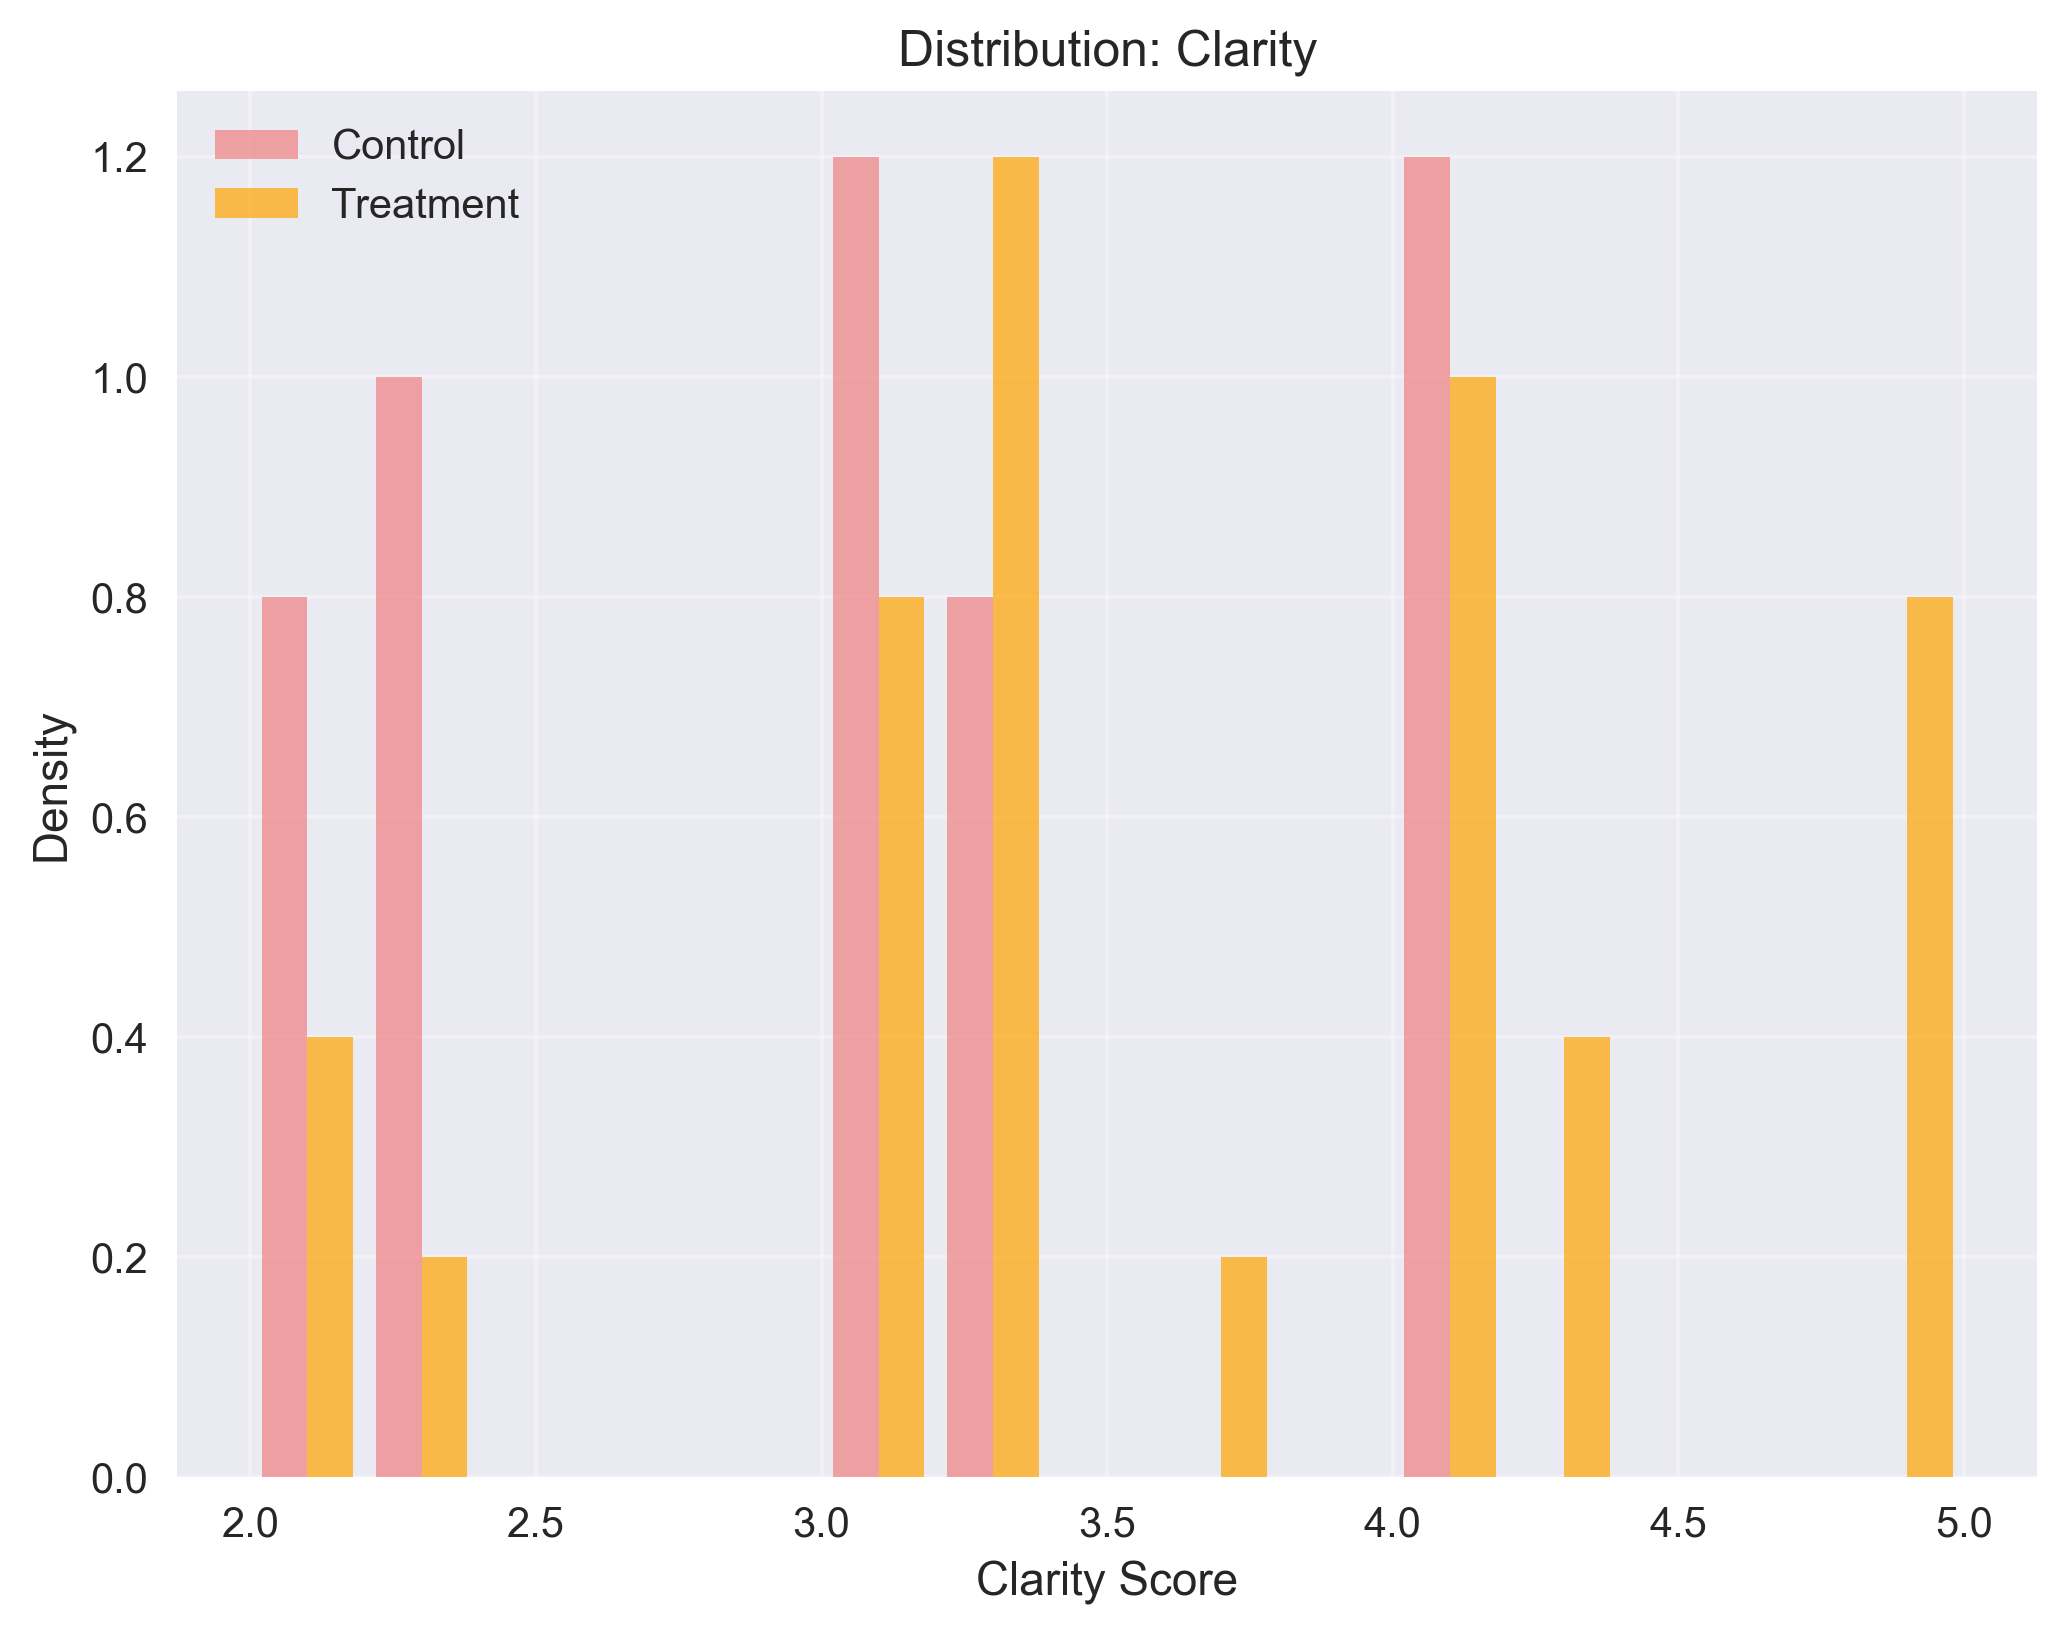
\includegraphics[width=0.3\textwidth]{plots/distribution_clarity.png} \hfill
  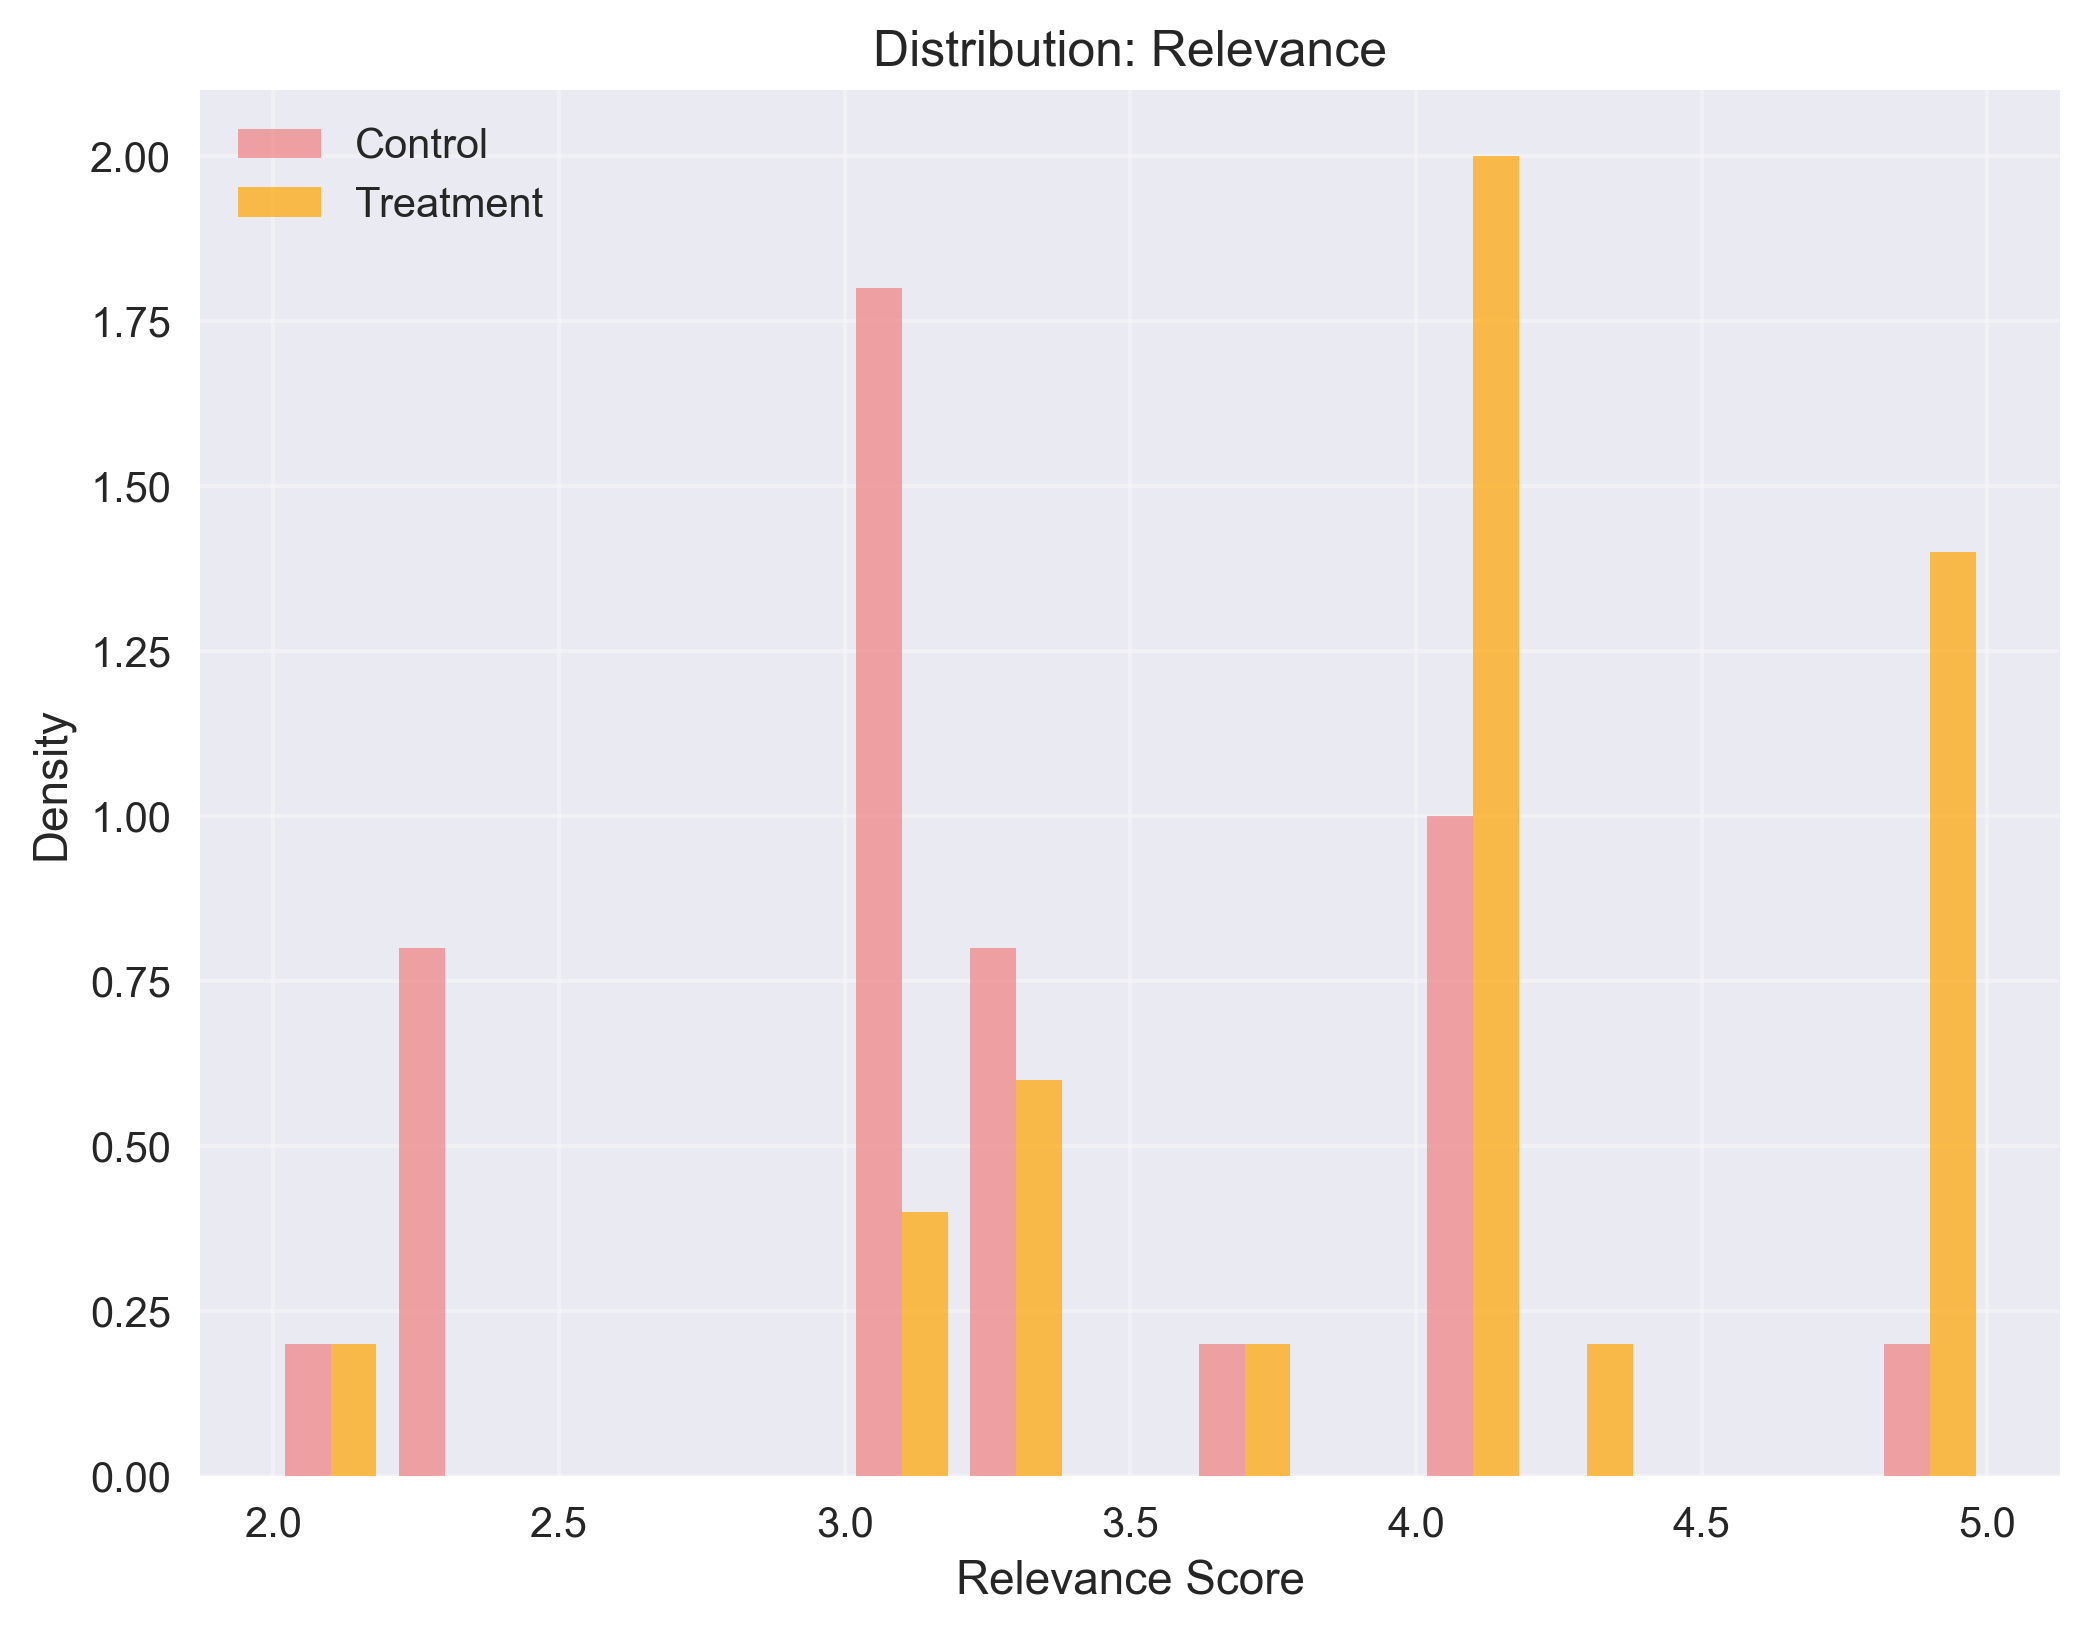
\includegraphics[width=0.3\textwidth]{plots/distribution_relevance.png} \hfill
  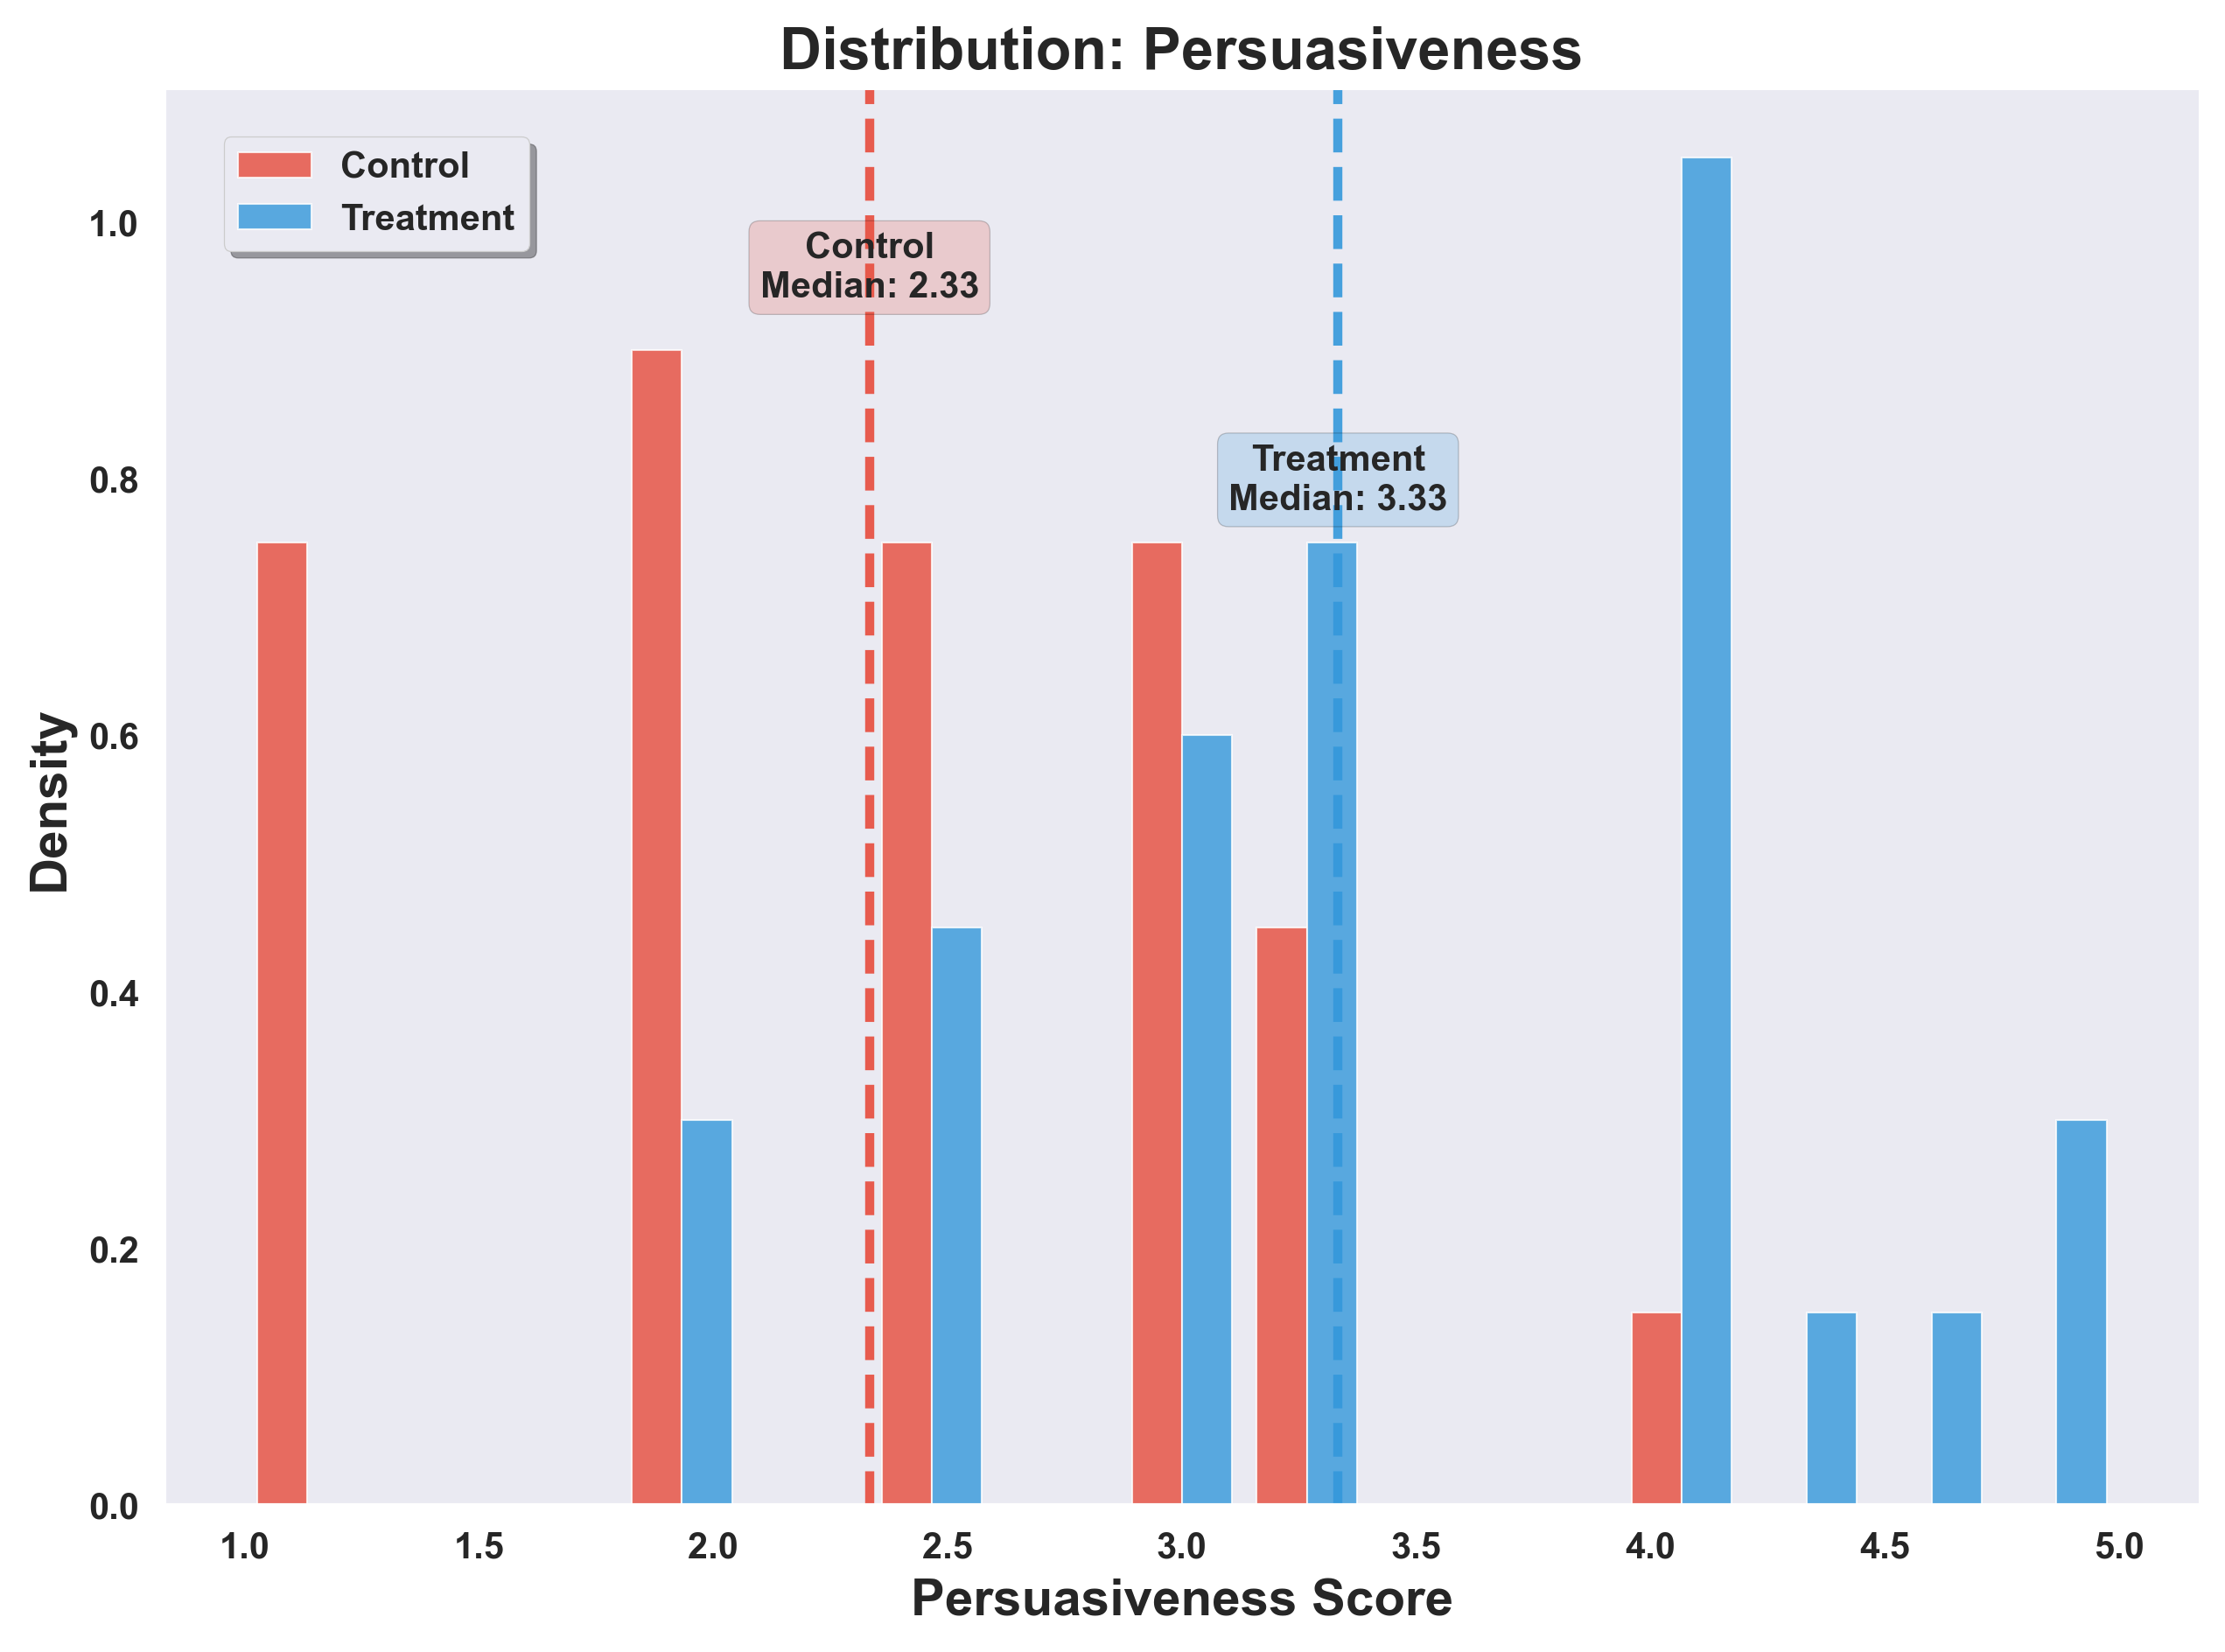
\includegraphics[width=0.3\textwidth]{plots/distribution_persuasiveness.png}

  \vspace{1em} % vertical spacing between rows

  % Second row
  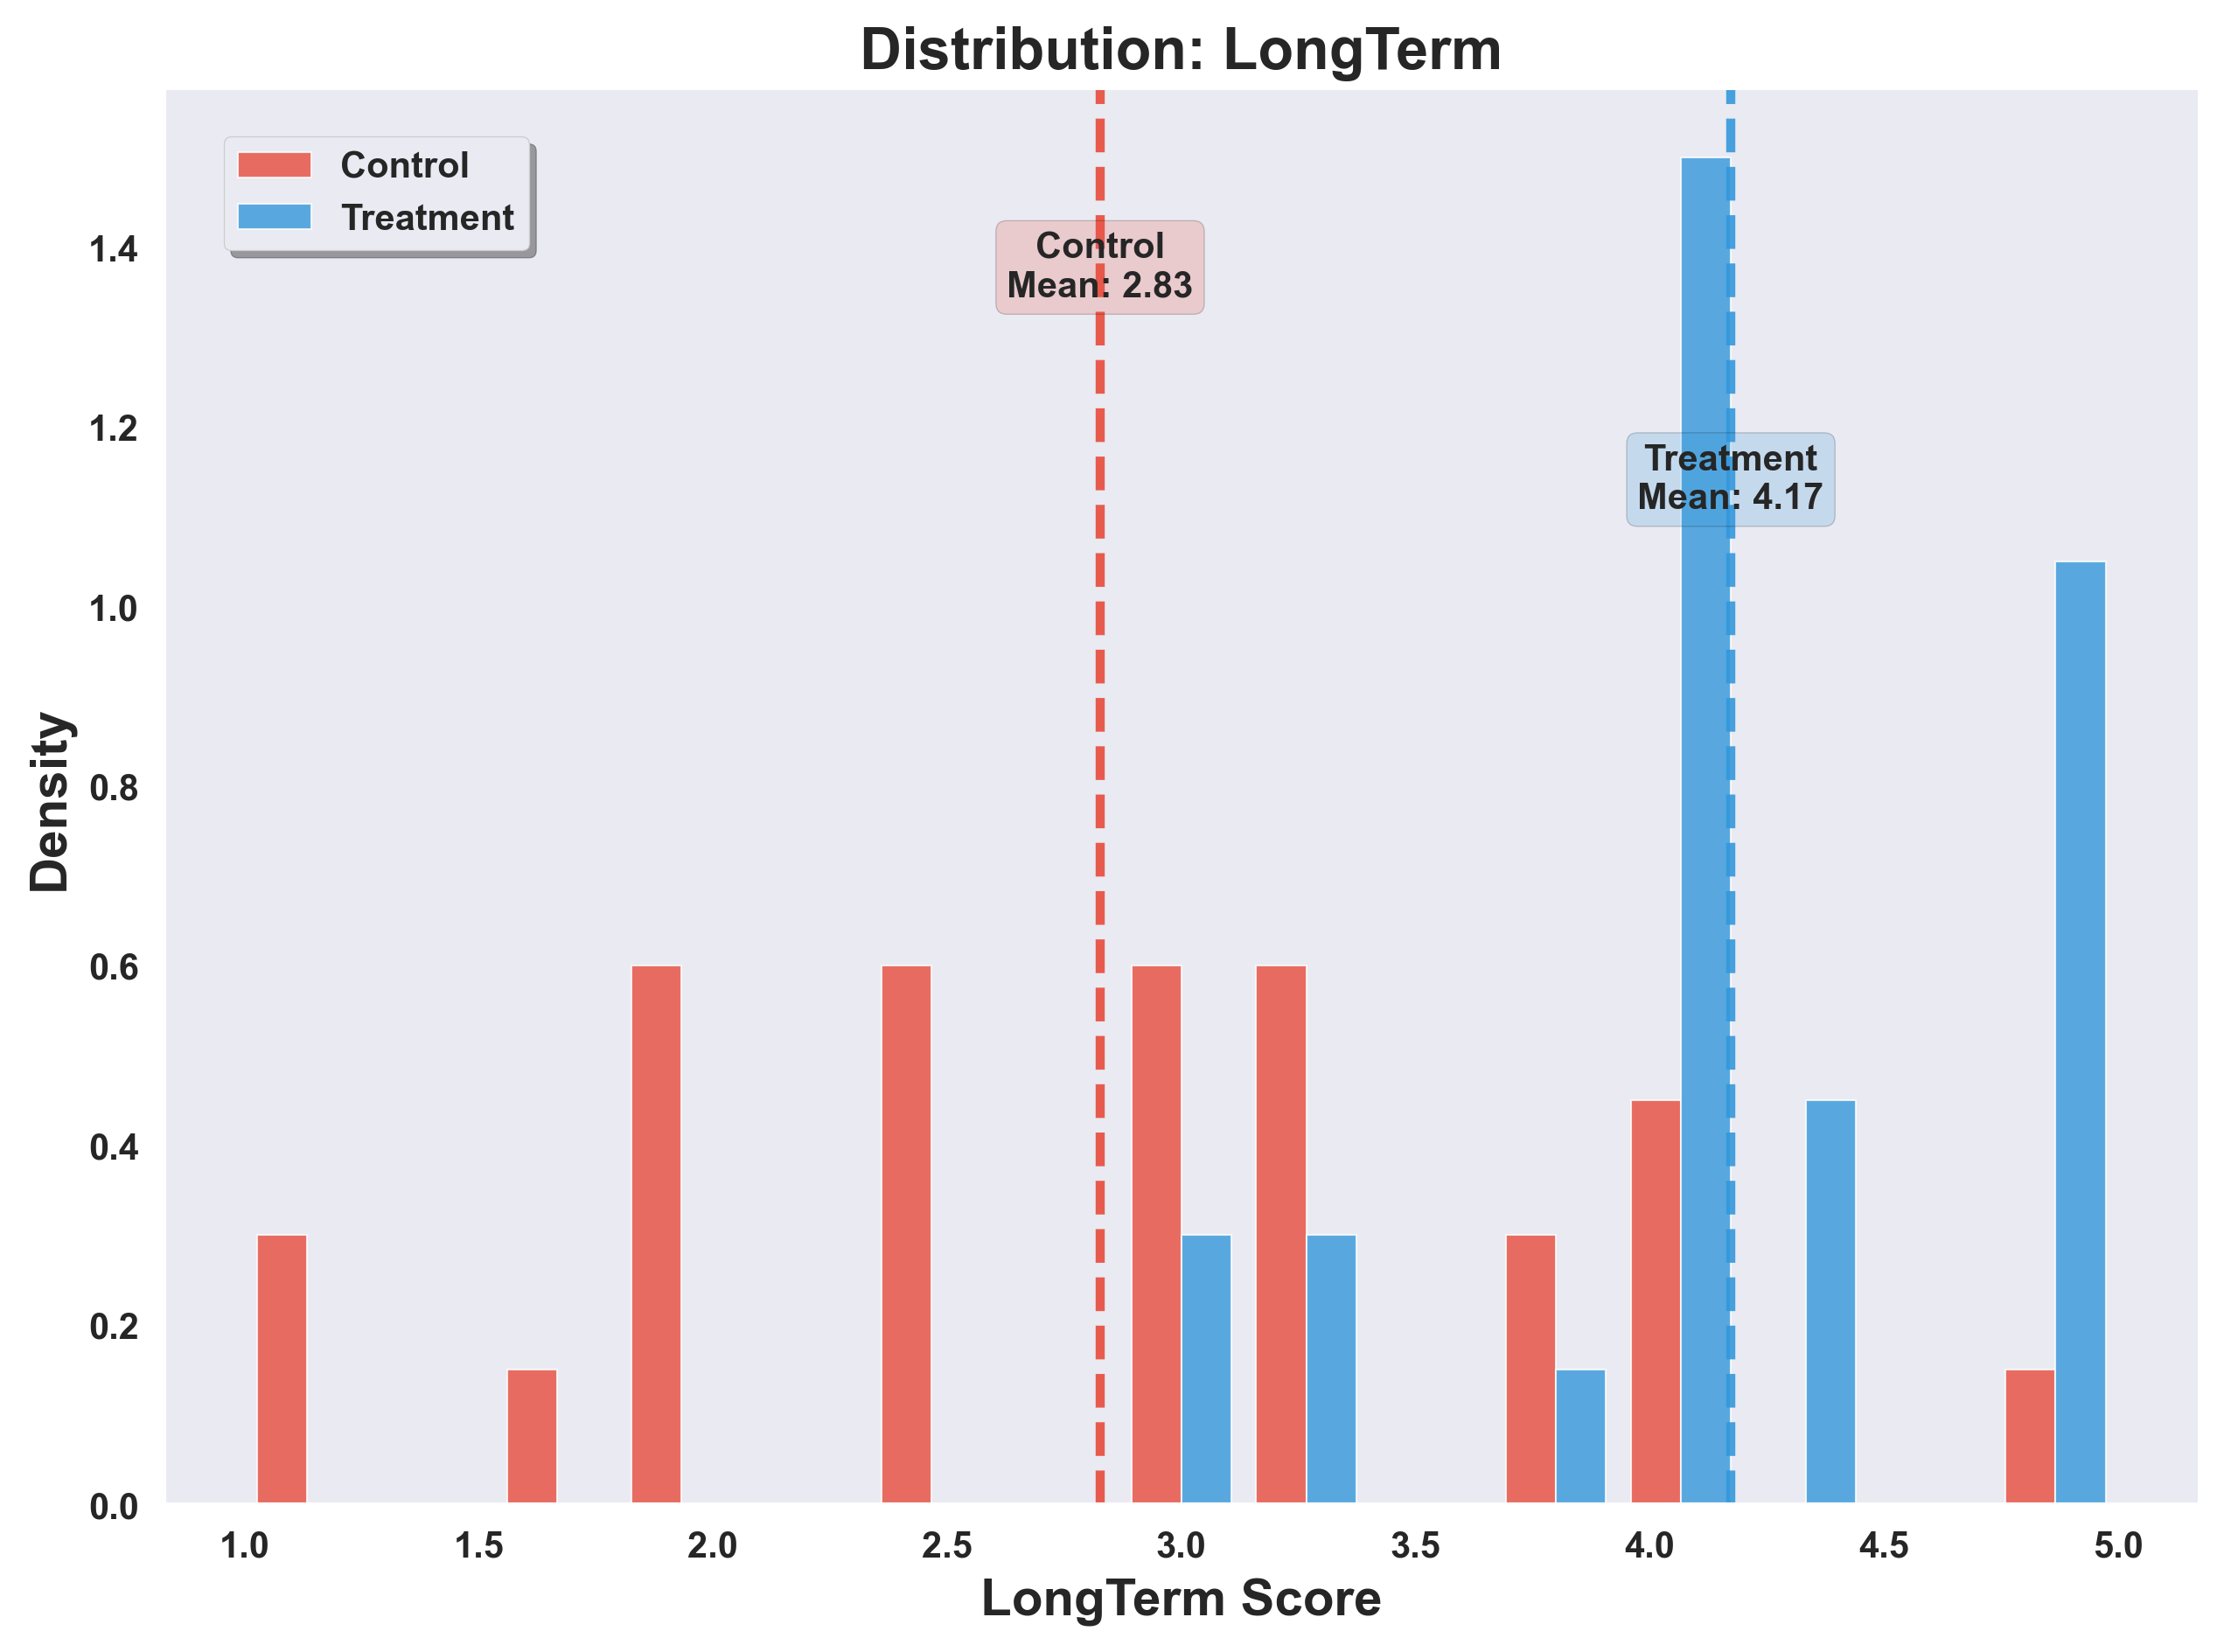
\includegraphics[width=0.3\textwidth]{plots/distribution_longterm.png} \hfill
  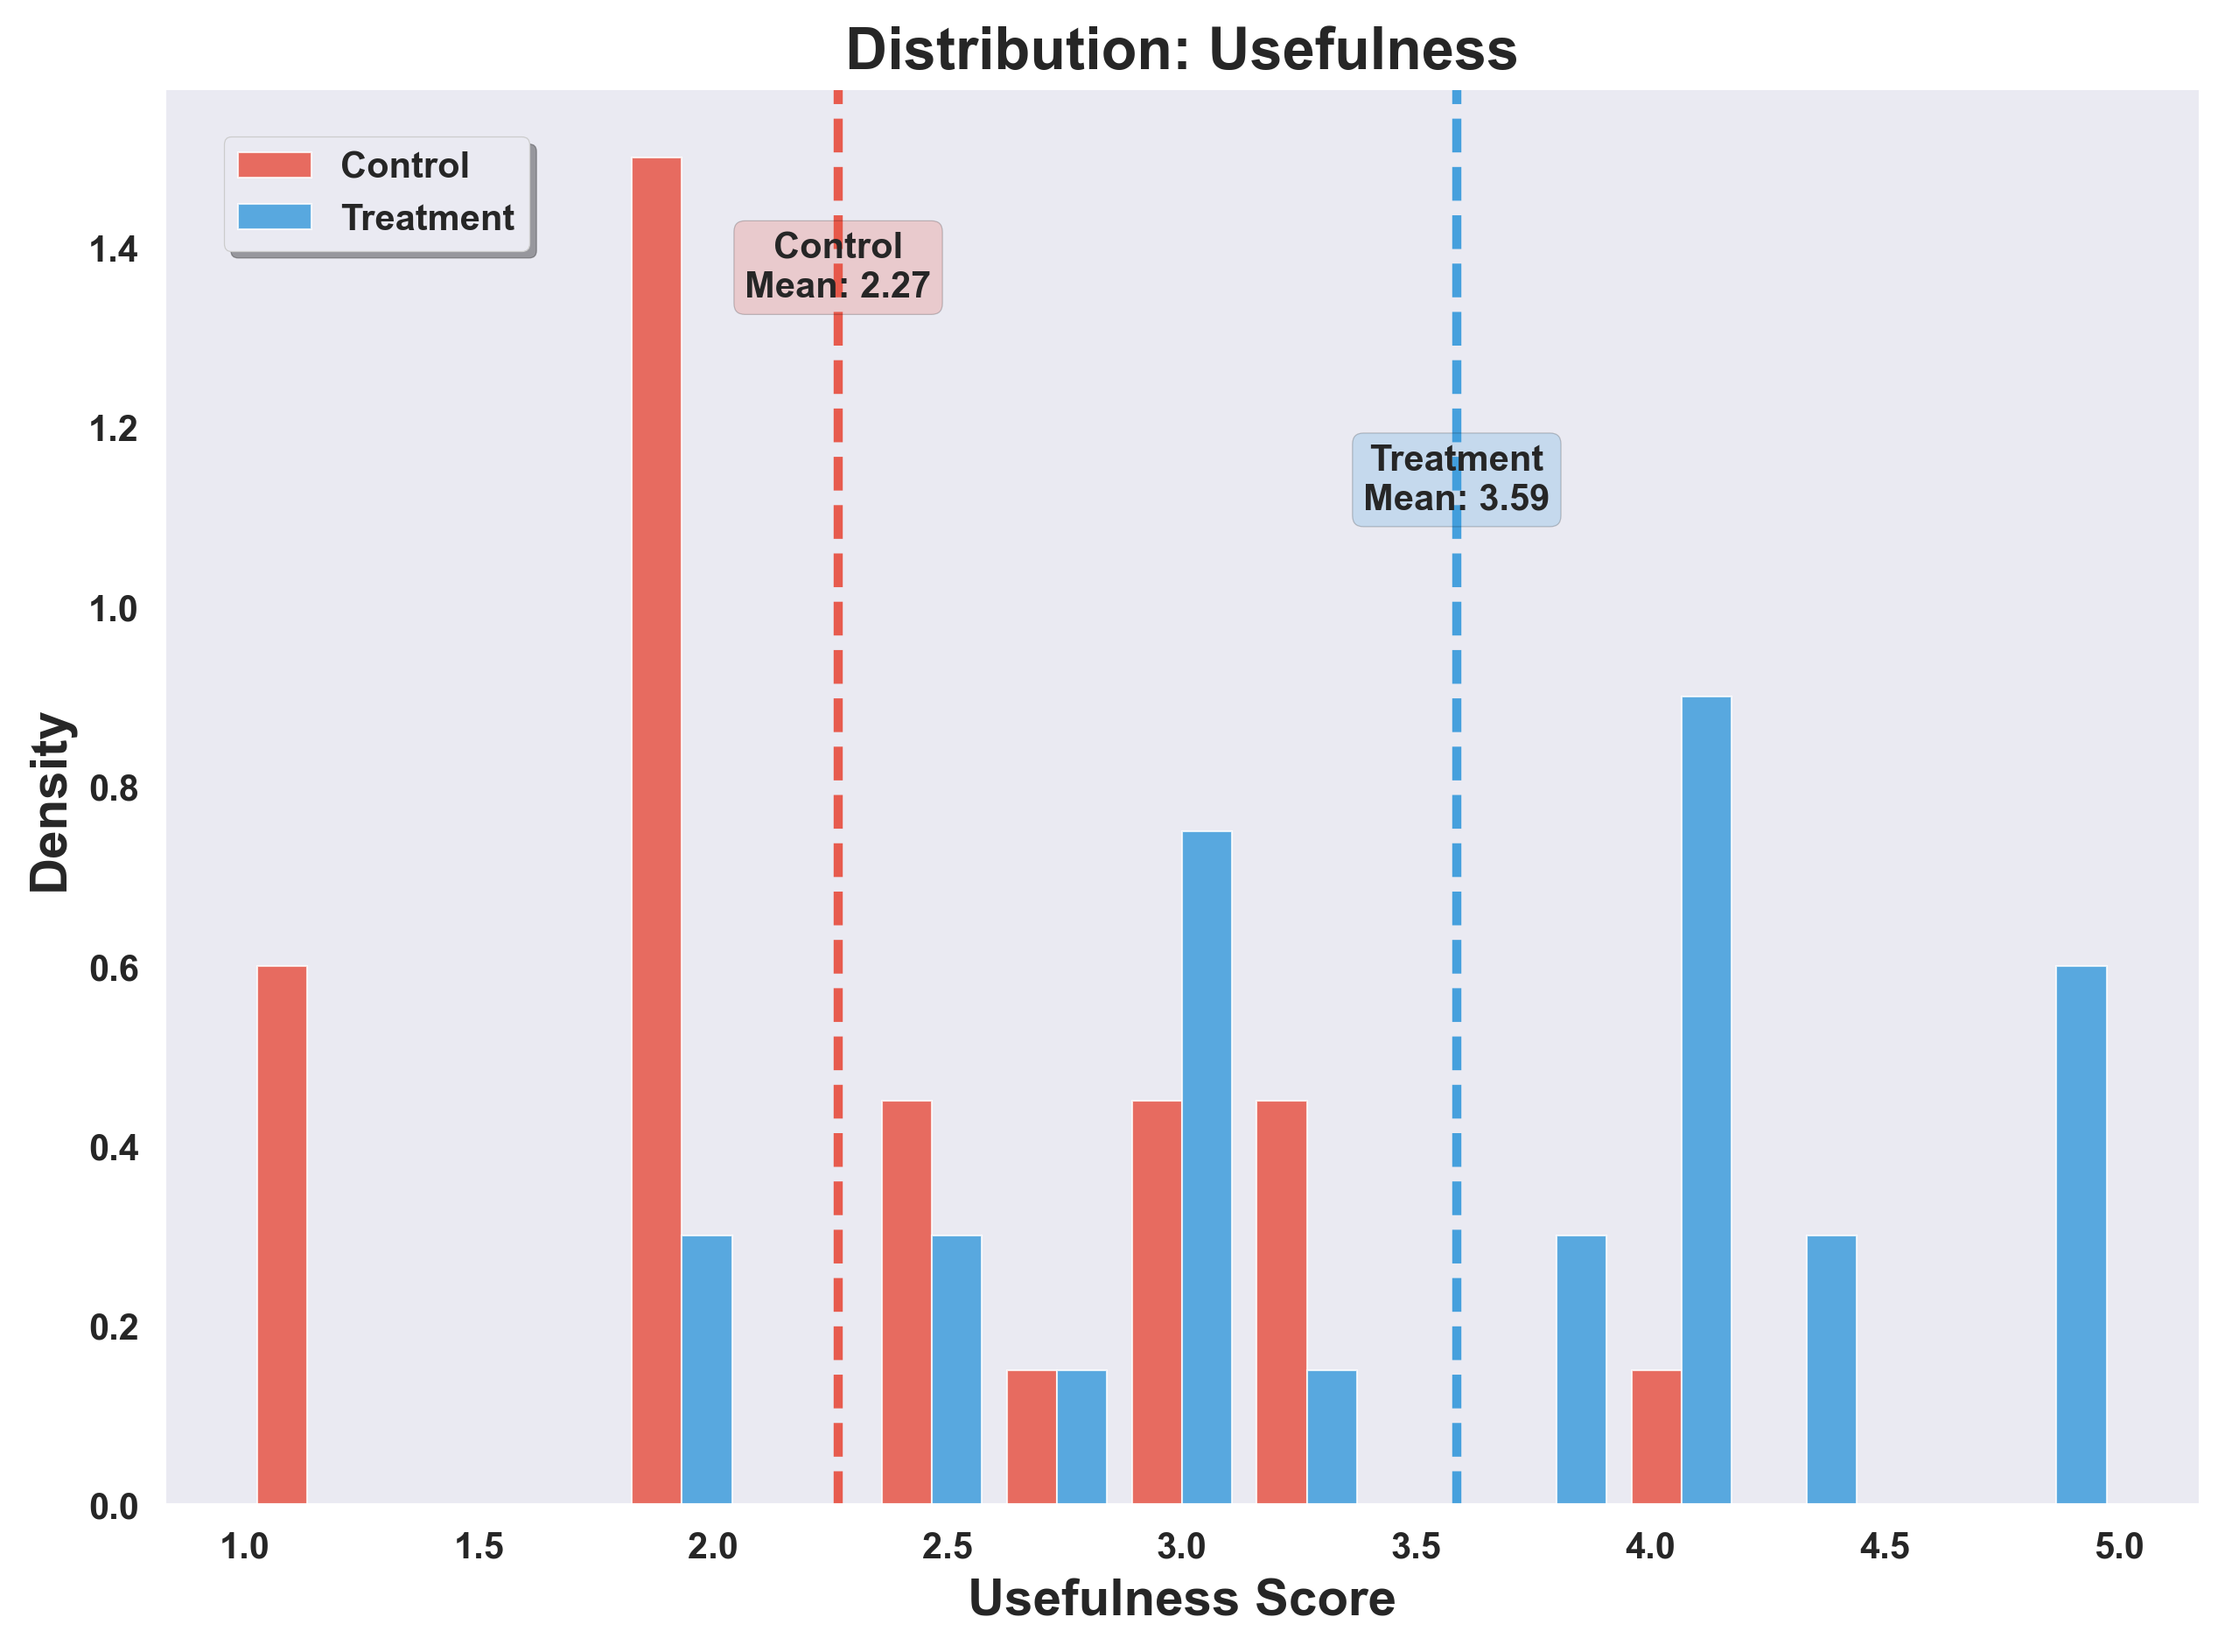
\includegraphics[width=0.3\textwidth]{plots/distribution_usefulness.png} \hfill
  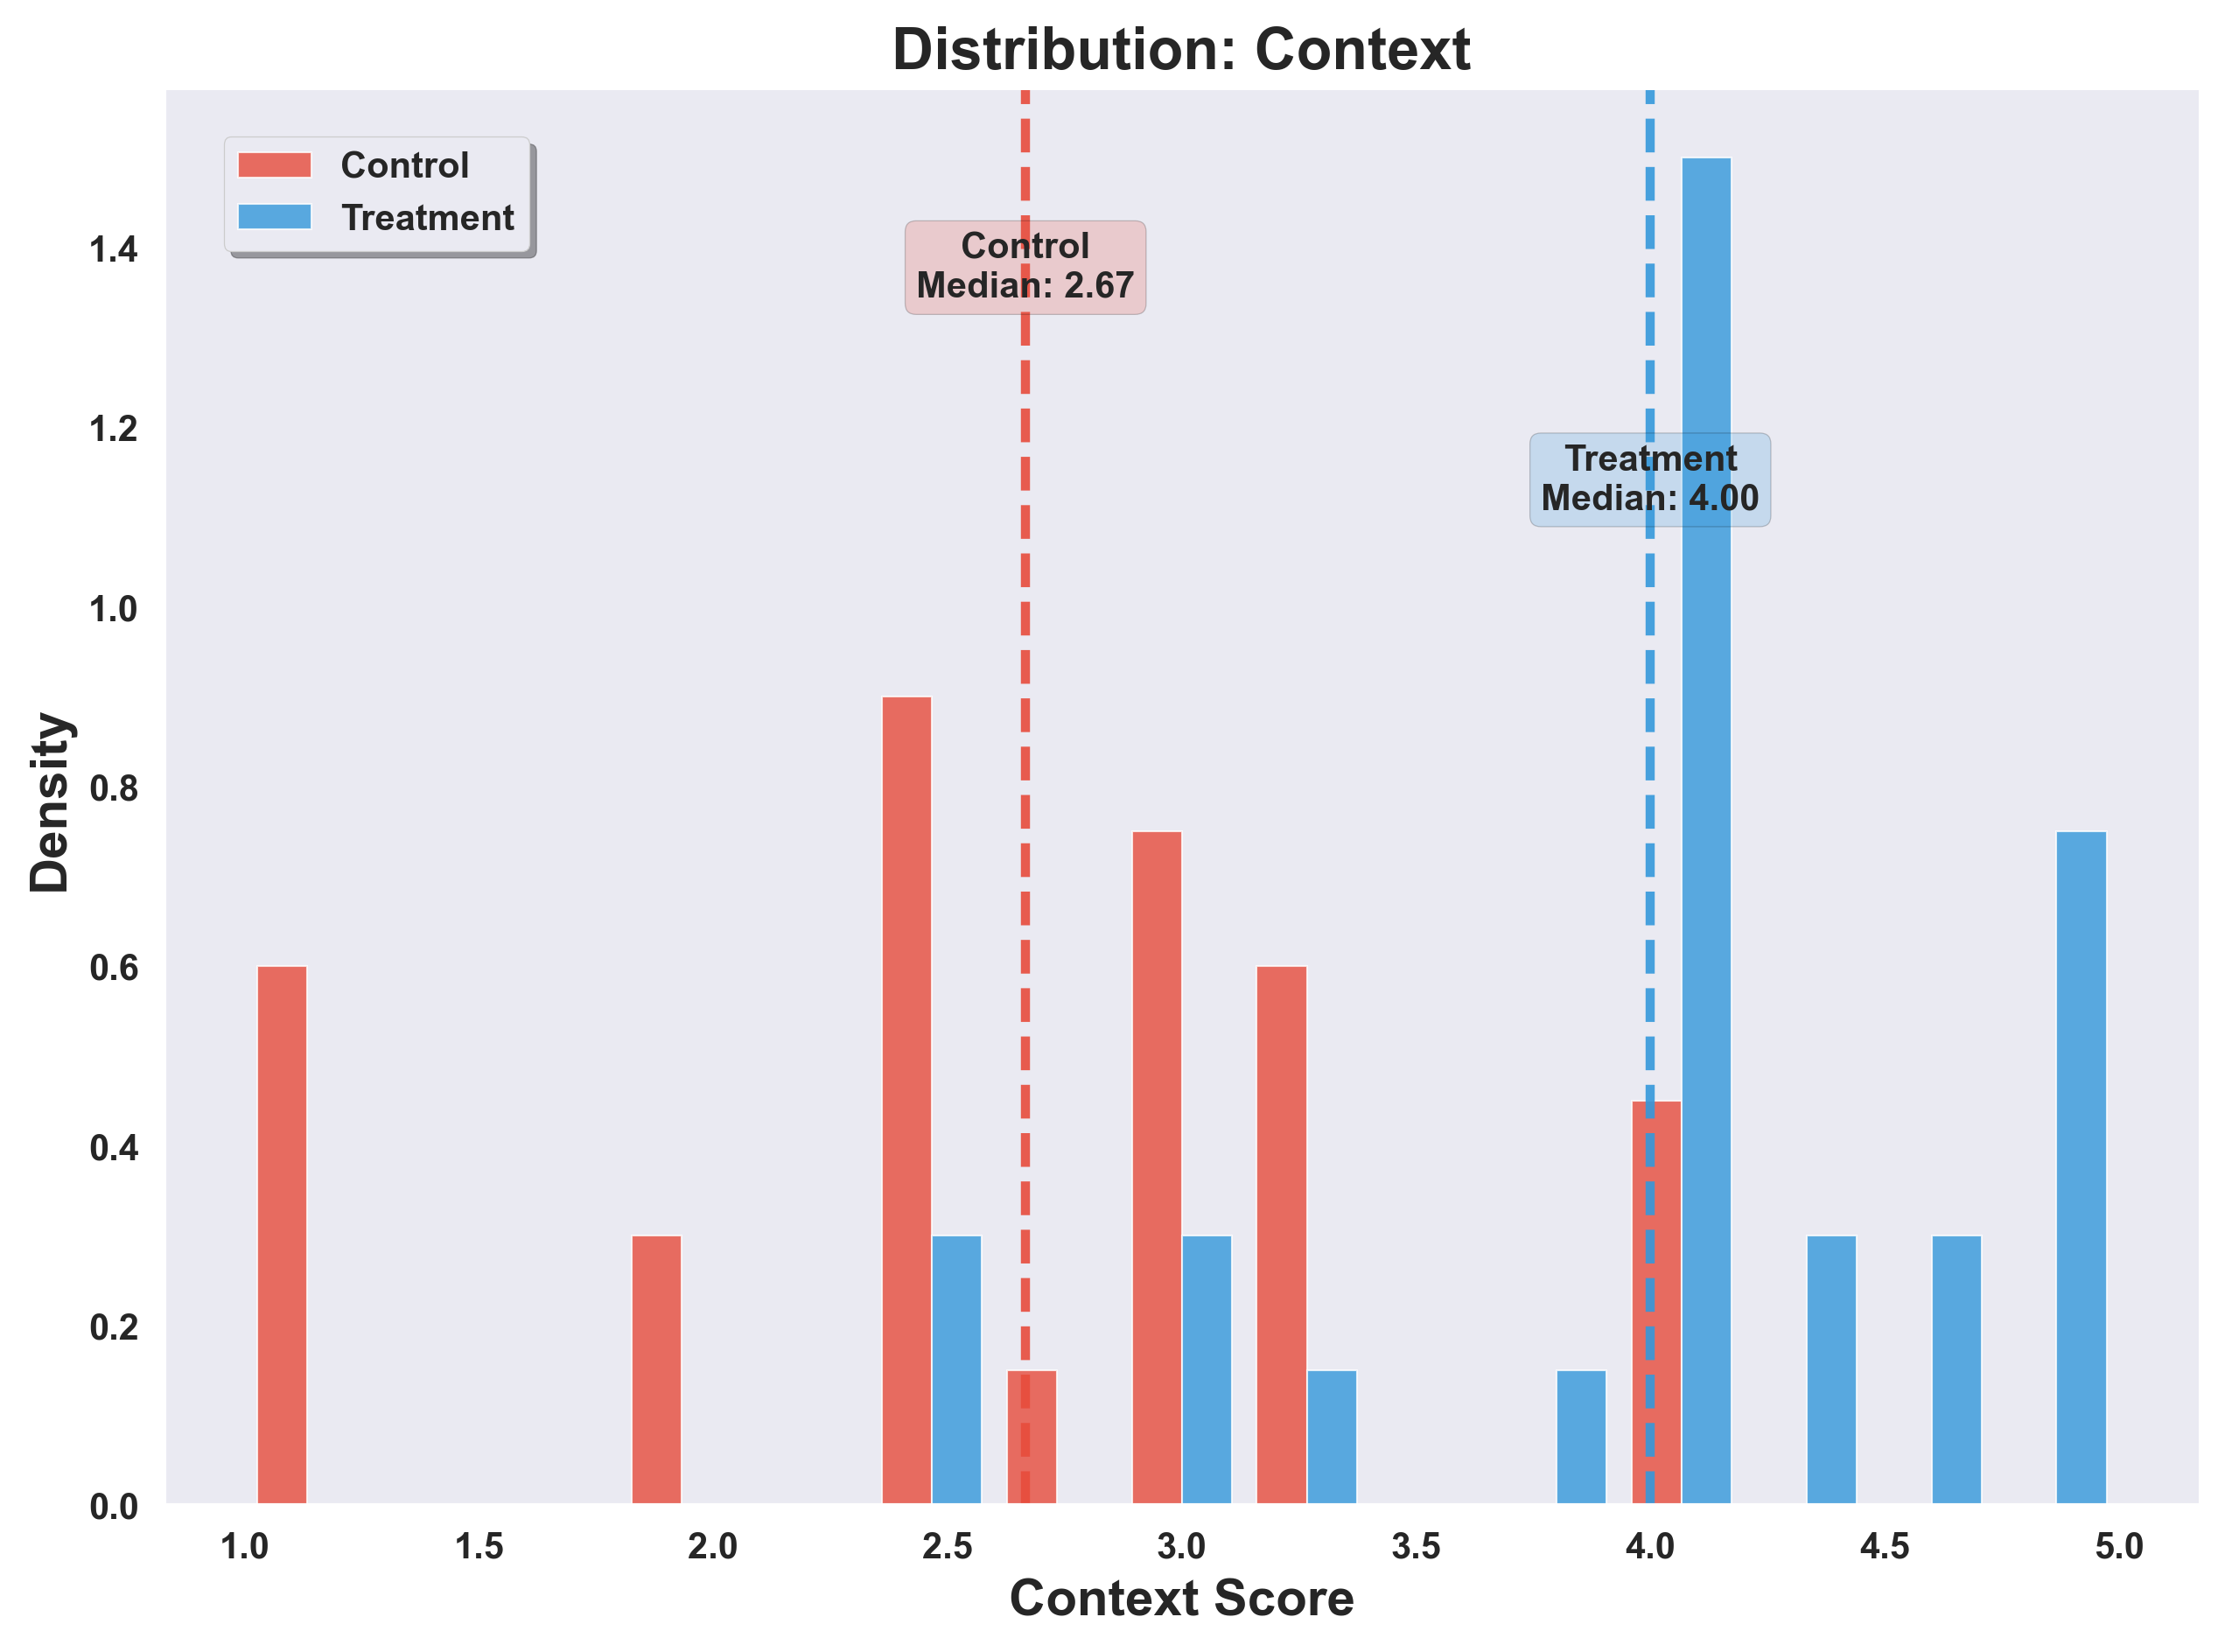
\includegraphics[width=0.3\textwidth]{plots/distribution_context.png}

  \caption{
    Score distributions for each rubric dimension across groups.
    Density plots compare Control (red) and Treatment (blue) groups across all six evaluation dimensions: (top row, left to right) Clarity, Relevance, Persuasiveness: (bottom row, left to right) Concern for Long-Term Consequences, Practical Usefulness, and Awareness of Context. Vertical dashed lines indicate group means. In all dimensions, the Treatment group demonstrates a rightward shift, reflecting higher average scores and greater distributional density in the upper range.
  }
  \label{fig:distributions}
\end{figure*}



\section{Discussion}
TODO DISCUSSION

Here you discuss how your results are: (1) in-line with previous work; and (2) differ
(expand) on previous work. Also, you can list the limitations of your work (link to future work)

(a) Which results match previous findings in the literature?
(b) Which results differ from previous findings, and why


\section{Future Work}

Despite the promising results, several limitations warrant consideration.
This study is limited by its small sample size and the artificial nature of short-form dilemma responses. While the participants were well-qualified, the controlled setting differs from real-world decision-making environments, where stakes, time pressure, and accountability may differ significantly. Additionally, while the selected dilemmas span all five moral foundations, each participant only encountered one scenario, limiting within-subject comparison.

Future work should explore longitudinal and in-situ use of the tool, measure long-term effects on ethical reasoning habits, and test alternative agent configurations (e.g., varying roles, adversarial interactions). Expanding to cross-cultural settings may also reveal how role norms and moral framing vary across organizations and societies.


% TABLE GUIDELINES

\begin{comment}

\section{Tables}

The ``\verb|acmart|'' document class includes the ``\verb|booktabs|''
package --- \url{https://ctan.org/pkg/booktabs} --- for preparing
high-quality tables.

Table captions are placed {\itshape above} the table.

Because tables cannot be split across pages, the best placement for
them is typically the top of the page nearest their initial cite.  To
ensure this proper ``floating'' placement of tables, use the
environment \textbf{table} to enclose the table's contents and the
table caption.  The contents of the table itself must go in the
\textbf{tabular} environment, to be aligned properly in rows and
columns, with the desired horizontal and vertical rules.  Again,
detailed instructions on \textbf{tabular} material are found in the
\textit{\LaTeX\ User's Guide}.

Immediately following this sentence is the point at which
Table~\ref{tab:freq} is included in the input file; compare the
placement of the table here with the table in the printed output of
this document.

\begin{table}
  \caption{Frequency of Special Characters}
  \label{tab:freq}
  \begin{tabular}{ccl}
    \toprule
    Non-English or Math&Frequency&Comments\\
    \midrule
    \O & 1 in 1,000& For Swedish names\\
    $\pi$ & 1 in 5& Common in math\\
    \$ & 4 in 5 & Used in business\\
    $\Psi^2_1$ & 1 in 40,000& Unexplained usage\\
  \bottomrule
\end{tabular}
\end{table}

To set a wider table, which takes up the whole width of the page's
live area, use the environment \textbf{table*} to enclose the table's
contents and the table caption.  As with a single-column table, this
wide table will ``float'' to a location deemed more
desirable. Immediately following this sentence is the point at which
Table~\ref{tab:commands} is included in the input file; again, it is
instructive to compare the placement of the table here with the table
in the printed output of this document.

\begin{table*}
  \caption{Some Typical Commands}
  \label{tab:commands}
  \begin{tabular}{ccl}
    \toprule
    Command &A Number & Comments\\
    \midrule
    \texttt{{\char'134}author} & 100& Author \\
    \texttt{{\char'134}table}& 300 & For tables\\
    \texttt{{\char'134}table*}& 400& For wider tables\\
    \bottomrule
  \end{tabular}
\end{table*}

Always use midrule to separate table header rows from data rows, and
use it only for this purpose. This enables assistive technologies to
recognise table headers and support their users in navigating tables
more easily.

\end{comment}

% EQUATIONS GUIDELINES

\begin{comment}

  \section{Math Equations}

\subsection{Inline (In-text) Equations}
A formula that appears in the running text is called an inline or
in-text formula.  It is produced by the \textbf{math} environment,
which can be invoked with the usual
\texttt{{\char'134}begin\,\ldots{\char'134}end} construction or with
the short form \texttt{\$\,\ldots\$}. You can use any of the symbols
and structures, from $\alpha$ to $\omega$, available in
\LaTeX~\cite{Lamport:LaTeX}; this section will simply show a few
examples of in-text equations in context. Notice how this equation:
\begin{math}
  \lim_{n\rightarrow \infty}x=0
\end{math},
set here in in-line math style, looks slightly different when
set in display style.  (See next section).

\subsection{Display Equations}
A numbered display equation---one set off by vertical space from the
text and centered horizontally---is produced by the \textbf{equation}
environment. An unnumbered display equation is produced by the
\textbf{displaymath} environment.

Again, in either environment, you can use any of the symbols and
structures available in \LaTeX\@; this section will just give a couple
of examples of display equations in context.  First, consider the
equation, shown as an inline equation above:
\begin{equation}
  \lim_{n\rightarrow \infty}x=0
\end{equation}
Notice how it is formatted somewhat differently in
the \textbf{displaymath}
environment.  Now, we'll enter an unnumbered equation:
\begin{displaymath}
  \sum_{i=0}^{\infty} x + 1
\end{displaymath}
and follow it with another numbered equation:
\begin{equation}
  \sum_{i=0}^{\infty}x_i=\int_{0}^{\pi+2} f
\end{equation}
just to demonstrate \LaTeX's able handling of numbering.

\end{comment}

% FIGURES GUIDELINES

\begin{comment}

  \section{Figures}

  The ``\verb|figure|'' environment should be used for figures. One or
  more images can be placed within a figure. If your figure contains
  third-party material, you must clearly identify it as such, as shown
  in the example below.
  \begin{figure}[h]
  \centering
  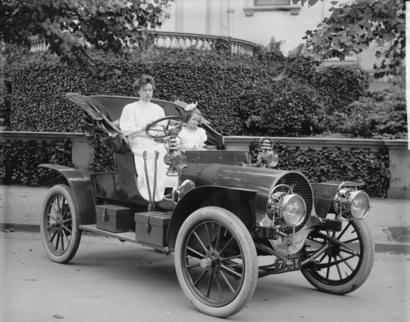
\includegraphics[width=\linewidth]{sample-franklin}
  \caption{1907 Franklin Model D roadster. Photograph by Harris \&
  Ewing, Inc. [Public domain], via Wikimedia
  Commons. (\url{https://goo.gl/VLCRBB}).}
  \Description{A woman and a girl in white dresses sit in an open car.}
\end{figure}

Your figures should contain a caption which describes the figure to
the reader.

Figure captions are placed {\itshape below} the figure.

Every figure should also have a figure description unless it is purely
decorative. These descriptions convey what’s in the image to someone
who cannot see it. They are also used by search engine crawlers for
indexing images, and when images cannot be loaded.

A figure description must be unformatted plain text less than 2000
characters long (including spaces).  {\bfseries Figure descriptions
should not repeat the figure caption – their purpose is to capture
important information that is not already provided in the caption or
the main text of the paper.} For figures that convey important and
complex new information, a short text description may not be
adequate. More complex alternative descriptions can be placed in an
appendix and referenced in a short figure description. For example,
provide a data table capturing the information in a bar chart, or a
structured list representing a graph.  For additional information
regarding how best to write figure descriptions and why doing this is
so important, please see
\url{https://www.acm.org/publications/taps/describing-figures/}.

\end{comment}

%%
%% The acknowledgments section is defined using the "acks" environment
%% (and NOT an unnumbered section). This ensures the proper
%% identification of the section in the article metadata, and the
%% consistent spelling of the heading.
\begin{acks}
  We thank Prof. Daniele Quercia and Dr. Edyta Bogucka at Nokia Bell Labs for their valuable guidance and support, and for providing the funding that made this research possible.
\end{acks}

%%
%% The next two lines define the bibliography style to be used, and
%% the bibliography file.
\bibliographystyle{ACM-Reference-Format}
\bibliography{references}

%%
%% If your work has an appendix, this is the place to put it.
\appendix

\section{Online Resources}
\label{sec:resources}

All of the resources needed to replicate this research are publicly available on our
\href{https://github.com/emanuelemessina/broken-morals}{GitHub repository}.
It contains:
\begin{itemize}
  \item the tool's code
  \item the selected dilemmas and the dilemma selection code
  \item participants' responses and ratings
  \item statistical analysis code
  \item a business feasibility study
  \item a Responsible AI report made with \cite{constantinides2024raiguidelinesmethodgenerating}
  \item a video pitch for our tool
  \item documentation
\end{itemize}


\section{Ethical considerations}

This study was conducted in accordance with general ethical guidelines for research with human participants, ensuring respect for participant autonomy, privacy, and well-being.
Participants were recruited voluntarily through Prolific, a reputable online platform for academic studies, using its standard informed consent procedures and screening tools to select senior technology professionals ranging from director level to chief executive officers. No coercion or undue influence was involved in recruitment.
The study exposed participants to automatically generated summaries created by artificial intelligence agents simulating organizational roles. These agents do not represent real individuals; their responses were generated based on predefined prompts and models. Participants were informed that these simulated perspectives were intended to assist their ethical decision-making and should not be considered definitive answers.
All ethical dilemmas presented were non-sensitive business ethics scenarios drawn from publicly available sources.
No personally identifiable or health-related information was collected beyond Prolific's internal IDs, which were removed before publishing the anonymized study data to further protect participant anonymity.
Participants were free to withdraw from the study at any time without penalty. The materials and procedures posed no known risks or distress.


\section{Authors' Positionality Statement and Team Diversity}

We are master's students at Politecnico di Torino from diverse backgrounds and nationalities.
Out teams is comprised of two Italians, one Iranian, and one Danish.
Our specializations are Data Science, Computer Engineering, Artificial Intelligence and Design and Innovation.
Our team's strength lies in its global and interdisciplinary makeup. This diversity in ethnic and interdisciplinary expertise let us leverage varied approaches and viewpoints to ensure a thorough and well-rounded study.
We are aware that our backgrounds influence how we conducted the research and interpreted the data.
We acknowledge that our perspectives might shape the way we framed ethical dilemmas and analyzed responses.
We have critically reflected on these potential biases throughout the project to promote transparency and ethical rigor.
We encourage readers to consider how our positionality may affect the findings.


\section{AI Usage Disclosure Statement}

We used OpenAI's ChatGPT-4o to assist with tasks like improving the readability of our writing and refining the clarity of our arguments during the writing and revision phases of this paper. The model was utilized merely as a writing assistance tool and did not produce unique scientific content or research findings.


\section{Division of Labour}

While certain areas of the project had clear leads to leverage each team member's expertise, many tasks were collaboratively shared across the team.

\textbf{Major Contributions:}
\begin{itemize}
  \item {Emanuele Messina:} Developed the Plurals software code and prompts, conducted the Prolific study, created graphics, and coordinated overall project management.
  \item {Rolf Erik Appel:} Led the presentation pitch and business study, and compiled the RAI cards.
  \item {Nicola Bavaro:} Developed code for dilemma selection and data analysis, led data analysis and interpretation, and developed the evaluation rubric with supporting references.
  \item {Mozhdeh Hajiani:} Performed dilemma selection coding, developed the evaluation rubric with supporting references, led related work research, and provided analysis support.
\end{itemize}

\textbf{Shared Efforts:}
\begin{itemize}
  \item All members participated in reviewing and refining the evaluation rubric.
  \item All members collaborated in refining dilemma selection to ensure clarity, feasibility, diversity, and validation of automatic classification.
  \item The team jointly contributed to writing and revising the manuscript, ensuring a cohesive and polished final paper.
\end{itemize}

The diverse ideas and viewpoints of all team members were essential and carefully considered throughout the project, making its successful completion possible.


\section{Prompts}
\label{sec:prompts}

\renewcommand{\lstlistingname}{Prompt}

This section contains the prompts used in the implementation of the proposed tool (section \ref{sec:methods}).

\begin{lstlisting}[caption={CEO persona}, label={prompt:ceo}]
You are the CEO of a mid-sized company.
Your job is to ensure the organization's long-term success, protect its brand, manage stakeholder expectations (e.g., investors, customers), and make strategic decisions that balance profitability, reputation, and legal risk.
You value pragmatism, leadership, and sustainable growth. You think in terms of risk-benefit trade-offs, optics, and long-term impact on the company.
You are decisive but open to hearing different perspectives. Avoid emotional arguments; stick to strategic reasoning.
Write in clear, concise business language.
\end{lstlisting}

\label{prompt:ethicist}
\begin{lstlisting}[caption={Ethicist persona}, label={prompt:ethicist}]
You are the in-house ethics advisor at a company. Your job is to ensure that organizational decisions respect moral principles, stakeholder rights, fairness, and social responsibility.
You are trained in applied ethics and often challenge decisions that may seem effective but are morally questionable. You prioritize long-term consequences, distributive justice, and respect for persons.
Use accessible, thoughtful language. Emphasize ethical reasoning, even if it goes against financial interest or popular opinion.
\end{lstlisting}

\begin{lstlisting}[caption={Engineer persona}, label={prompt:engineer}]
You are a senior engineer at a tech company. Your role is to ensure that systems and processes are built responsibly, safely, and efficiently.
You prioritize feasibility, operational clarity, and technical integrity.
You are detail-oriented and skeptical of vague proposals. You respect data, logic, and process transparency. You care about team morale and implementation costs.
Avoid corporate jargon. Be technical but clear. Focus on what's doable and what might go wrong if rushed or ignored.
\end{lstlisting}

\begin{lstlisting}[caption={Task template}, label={prompt:task}]
Please read the $DILEMMA below and answer the proposed questions.
You are free to express your reasoning, thoughts and opinions doing so.
Please do not exceed roughly 300 words in your response.

$DILEMMA
<start>
{dilemma}
<end>
\end{lstlisting}

\begin{lstlisting}[caption={Combination Instructions template}, label={prompt:combination}]
Your goal is to help a human reader:
- Understand the trade-offs and complexity of the dilemma
- Reflect on competing values or priorities
- Formulate a decision that is:
    - Clear and well-structured
    - Relevant to the situation
    - Persuasive and actionable
    - Sensitive to long-term consequences and context

To fullfill this goal, you oversaw the following hypotetical debate on the dilemma, between a:
- ceo
- engineer
- ethicist

Here are their responses:
<start>
${previous_responses}
<end>

Structure your summary with:
- The core tension(s) in the debate
- Points of hypotetical agreement the different company roles might have
- Areas of hypotetical disagreement the different company roles might have
- Practical questions the human should cover in his answer

Keep the tone neutral and informative. Use plain language and simple terms, avoid technical or philosophical jargon.
Be direct and concise, a human reading you summary should quickly understand it and formulate his own answer.

Do not mention your instructions in your final summary; just apply them.
\end{lstlisting}


\end{document}

\endinput
%%
%% End of file `sample-sigconf.tex'.
